\documentclass[11pt,twoside,a4paper,openright]{report}
\usepackage{a4wide}


\usepackage[utf8]{inputenc}
\usepackage[english]{babel}
\usepackage{hyperref}
\usepackage{amsmath}

\usepackage{arydshln}

\usepackage{csquotes}

\usepackage[citestyle=numeric]{biblatex}
\bibliography{bibliography.bib}

\usepackage[noabbrev, capitalize]{cleveref}
\usepackage{siunitx}
\sisetup{per-mode = symbol}
\usepackage{nicefrac}
\usepackage[official]{eurosym}

\usepackage{amsmath}
\usepackage{mathtools}

\usepackage{fancyvrb}
\usepackage{listings}

\usepackage{algpseudocode}
\usepackage{algorithmicx}
\usepackage{algorithm}

\usepackage{tikz}
\usetikzlibrary{positioning,shapes,shadows,arrows,backgrounds, patterns, shapes.multipart, calc}
\usepackage{tikz-3dplot}

\usepackage{graphicx}
\graphicspath{{images/}}

\usepackage{caption}
\usepackage{subcaption}

\usepackage{longtable}
\usepackage{rotating}
\usepackage[tableposition=top]{caption}
\usepackage{tabu}
\usepackage{booktabs}

\begin{document}

\tableofcontents

\listoffigures
\listoftables

\newcommand{\TF}[2]{\prescript{#2}{#1}{\mathcal{T}}}


% \chapter{Introduction}

Digital reconstruction of three dimensional scenes is a field that gained a high importance in areas like architecture, robotics, archeology and autonomous driving. As an example, virtual reality technologies allows high-detail and high-resolution models to be experiences in an immersive 3D experience, and the technology is becoming available for the general public, as prices for this 3D headsets and VR-ready phones decrease. These new technologies create a demand for reconstruction technology and new algorithms that are accurate and of high quality.

\section{Motivation}

Despite all the work done, there is still no perfect solution. 3D reconstruction is still a challenge, because real scenes are very complex and measurements are subject to errors and noise. Past experience tells that a single sensor is not enough to model real environments, so currently the process lies into using multiple sensors and trying to merge the data from all the sensors, in order to capture a more realistic model.

However, this introduces a set of other problems inherent to this approach. For example, the data from different sensors needs to be merged accurately. Also, the positions of all the sensors need to be known accurately, which means that the calibration processes need to be more robust and precise.

Also, current reconstruction algorithms require a large amount of manual work, which means that a reconstruction require many man-hours to be completed, which is unfeasible for most applications. One of the goals of reconstruction is to develop algorithms that are automatic and do not require any intervention, making it faster and more accessible. 

An automatized reconstruction method is still a challenge today, but new algorithms could allow it, which would make reconstruction work more accessible.

Nowadays, 3D reconstruction software is even available in smartphones, usually targeting Augmented Reality applications. However, these 3D reconstructions are not accurate and the resulting models are far from perfect.

\section{Problem Description}

Nowadays, Lidar laser scanners are becoming more available and more accessible,  and because of their properties, as their high precision and high range, became an unmatched technology for 3D reconstruction. The lidar lasers are available as 2D laser scanners or 3D laser scanners, like the Velodyne. Despite their immense potential, 3D laser scanner is still a very expensive solution and cheaper solutions are comprised of a cheaper 2D laser scanner mounted on a moving frame. This solution, despite its low cost, can achieve good results, but requires a fine calibration. 

Also, laser scanners do not register the color information, so a common practice is to pair the laser scanner with a camera to get both geometric and color data. This method also requires a fine calibration between both sensors to correctly merge the data. 

\section{Objectives}

The objective is to develop a fully integrated solution for 3D acquisition using both laser and image data. This objective was divided into four main objectives.

The first objective was to develop a 3D laser scanner, consisting of a laser scanner and a camera, and capable of recording data from both sensors in a fast and semi-autonomous way.

The second objective was to define a methodology to record the data from the scene. This methodology should take into account the limitations of both sensors and try to minimize their effect in the final result.

The third objective was to develop a set of methods to reconstruct the geometry of the scene reliably. The main challenge is the extrinsic calibration of the laser, because it is fundamental for a reliable reconstruction. So, a new calibration method was developed to achieve the wanted results.

The fourth and final objective was to develop a set of methods to merge the image data with the geometry of the scene, to reconstruct the color.

The final result is then, a point cloud with color and geometric information.

\section{Document Outline}

This dissertation is composed of eight chapters, which are arranged as follows:

\begin{description}
    \item[Introduction] The current chapter, in which the description of the problem is shown and the objectives of this work are defined.
    \item[State of Art] Describes the technologies and solutions found in the field of 3D reconstruction, both commercial and academic, as well of a small technical background on this solutions.
    \item[Experimental Infraestructure] Introduces all the software and hardware used to develop this work. In particular, the mobile robot for 3D scanner is described.
    \item[Methodology for Scene Capture] Describes the methods and algorithms used to reconstruct the geometry of the scene, using the laser scan data recorded.
    \item[Methodology for Image Reconstruction] Describes the methods and algorithms used to reconstruct the color information of the scene, using the camera images recorded.
    \item[Result and Discussion] Presents and discusses the experimental results obtained in this work.
    \item[Conclusion and Future Work] Summarizes the overall work developed and present possible future work.
\end{description}
% \chapter{State of Art}

\section{Technologies}

Many technologies were developed to capture tridimensional information of the environment. The following section describes such systems and describe the basic working principle along with the pros and cons inherent to each ones. These techniques can be categorized into triangulation and time-of-flight.

\subsection{Stereoscopy}

For many years, stereoscopy remained the most popular method for 3D sensing, also because its working principle resembles the human stereoscopic vision. This system uses images taken from a pair of cameras and extracts depth information using the perspective projection: the position of objects closer differ more than objects farther. To compute depth, features from both images are extracted and matched together, which makes it a complex and computationally demanding, so it requires fast computers or dedicated software. This system has the advantage of having a good rate of acquisition and having high resolution. Also, color information is available. However, the reconstruction algorithm rely heavy on environment characteristics, like lightning conditions, texture and non-homogeneous regions~\cite{klimentjew2010}. This means that this method gives good results for edges and textured areas, but fails to get the depth information of continuous surfaces. Also, the poor geometric precision is one of the limitation of this system.

\subsection{Structured Light}

In 2010, the availability of consumer grade depth sensors based on structured light lead to the development of consumer-grade small factor RGB-D cameras, started by Microsoft, with the \textit{Kinect} and followed by other devices, like \textit{ASUS Xtion} and \textit{Intel RealSense}. These cameras come in small form factors, are inexpensive and are capable of capturing both color and depth information at real-time rates~\cite{zollhoefer2018}.

These appealing characteristics lead to a huge research and development in 3D reconstruction using this camera, culminating in the KinectFusion algorithm \cite{kinectfusion2011}, capable of a fast and precise 3D reconstruction using a \textit{Kinect} RGB-D camera and commodity GPUs. This algorithm was capable of performing real-time reconstruction, using a Iterative Closest Point (ICP) for tracking the location of the device and for the registration of new RGB-D data. Nowadays, it is possible to achieve the same result using a phone equipped with a depth camera, like the \textit{Lenovo Phab 2} or \textit{ASUS Zenphone VR} and with the \textit{Google Tango} software. 

Structured light sensors work by projecting an infrared pattern onto the scene and calculate the depth via the perspective deformation of the pattern due to the different object's depth. However, this technique yields sub-optimal results: the depth values from structured light have significant error or can be missing, specially from objects with darker colors, specular surfaces or small surfaces~\cite{shen2013}. 

\subsection{Time of Flight}

Time of flight sensors, or ToF sensors, use the speed of light to measure the distance. A scene is illuminated by a light source and the reflected light is detected back by the sensor. The time that the light has taken to travel forth and back is then measured and the depth is calculated with this time. The measurement dependes on the type of ToF system used, that is ether \textit{continuous} or \textit{pulsed}. In \textit{pulsed} systems, light is emitted in bursts with a fast shutter and the time between the emission and the reception is calculated. \textit{Continuous} systems use a modulated light source and measure the phase-shift between the outgoing and incoming wave.

This technology has some advantages comparing to both previous approaches \cite{zollhoefer2018}. First, it is less computationally intensive, because the measurement is directly done by a specialized sensor. Second, it is partially independent of the lightning conditions because the light detected is emitted by the device itself. Further, it is capable of providing a dense and accurate depth values, even for continuous or irregular surfaces, unlike the stereoscopic approach. Moreover, it is much faster that any other method, capable of acquisition rates of hundreds of \si{\hertz}. However, it has some disadvantages as well. Unlike stereoscopic, which is a passive method, ToF sensors interact with the scene, so are not possible to be implemented in certain environments. Also, the properties of the material, like the reflectivity, color and roughness can have significant effects on the accuracy of ToF sensors. Moreover, multi-path reflections are a common problem of ToF sensors, caused by multiple reflections of the light, causing errors in the measurements. Furthermore, interference can exist if multiple ToF sensors share the same environment. However, it is possible to mitigate this effect, by either controlling the sensor such that only one is activate at a time, or by using different modulation frequencies in their illumination source.

A popular ToF sensor nowadays is the Photonic-Mixer-Device camera, which looks similarly to a normal image sensor, but measures the phase shift of incoming light. This sensor is now being used in new generation RGB-D cameras, replacing the structured light approach, mainly because it is more resilient to background light, allowing the sensor to work in outdoor environments \cite{zollhoefer2018}. One of this example is the new \textit{Kinetic 2}, that replaced the last depth sensor with this one.

\subsection{LiDAR}

Light Detection and Ranging, or LiDAR, is one of the most precise and reliable ways to measure distances. It began being used shortly after the invention of Laser, in 1960, and it's valuable characteristics lead to the integration of it in the Apollo 15 mission, to serve as an altimeter to map the surface of the moon. Soon after, it was implemented in aircrafts to create high-precision and dense earth's surface models. Nowadays, its applications can be found everywhere where an accurate distance measurement is required, as for example in geology, archeology, geography and meteorology.

The success of LiDAR is related to the use of laser as its light source. Lasers are capable of emitting beams of light that are monochromatic, narrow and polarized. That is, lasers emit light in a narrow spectrum, so they can produce a single color of light, also known as monochromatic light. It improves the resilience against background light, making it possible to use even with sun light. Also, laser photons travel parallel, creating a narrow beam that stays narrow even at large distances, with minimum scattering, therefore measuring the distance in a very small area in the surface. This improves the measurements near sharp transitions, where a bigger area of measurement can cause errors in the measurement. Moreover, lasers can transition between an on-off state in a very short time. This is significant to reduce the error of the distance measurement, because it is directly influenced by the time between pulses, and a sharp transition reduces the error in the time measurement. 

The first major application of LiDAR technology was to map and reconstruct the topology of the earth's surface. To do it, high range laser scanners are mounted on a plane and are flown above the target area. This is possible due to their high power laser, which allows ranges in the kilometer range, while maintaining precision in the centimeter range. This lasers also have a high sampling rate, in the order of the kilohertz, which is essencial to maintain a dense sampling, even at high travelling speeds. This high sampling also allows the terrain to be mapped even with high vegetation, because even that only a small percentage of points reach the terrain, there are still a significant number of points. This is just not possible with other methods, like aerial photography. 

Moreover, airborne LiDAR is also used to detect and classify clouds, which is an important data in meteorology. This is possible by studying the rayleigh scattering effect, which occurs when a laser beam goes through a particles smaller that its wave length, as for example, the water molecules in clouds.  This is essential for modern forecast prediction.

A airborne LiDAR scanner of the Austrian city Retz is shown in \cref{fig:riegl-lidar-scan}\footnote{In \url{http://www.potree.org/potree/examples/showcase/retz.html}.}, taken with a Riegl laser scanner placed in a Unmanned Aerial Vehicle. \cref{fig:riegl-lidar-scan-big} shows the entire scan with an area of \SI{1300 x 1300}{\meter}, \cref{fig:riegl-lidar-scan-small} shows a portion correspondent to the city, and \cref{fig:riegl-lidar-scan-tiny} shows the town hall, which has an area of about \SI{150 x 70}{\meter}. As can be seen, the result is a massive point cloud that covers a large area while still maintaining a high point density so small details are not smeared out. 

\begin{figure}[p]
    \centering
    \begin{subfigure}{\textwidth}
        \centering
        \includegraphics[width=.65\textwidth]{riegel-lidar-scan-big}
        \caption{The entire scan.}
        \label{fig:riegl-lidar-scan-big}
    \end{subfigure}

    \centering
    \begin{subfigure}{\textwidth}
        \centering
        \includegraphics[width=.65\textwidth]{riegel-lidar-scan-small}
        \caption{Pormenor of the City.}
        \label{fig:riegl-lidar-scan-small}
    \end{subfigure}

    \centering
    \begin{subfigure}{\textwidth}
        \centering
        \includegraphics[width=.65\textwidth]{riegel-lidar-scan-tiny}
        \caption{Pormenor of the Town Hall.}
        \label{fig:riegl-lidar-scan-tiny}
    \end{subfigure}

    \caption{Point cloud of Retz obtained by an airborne LiDAR.}
    \label{fig:riegl-lidar-scan}
\end{figure}

In recent years, LiDAR scanner became a fundamental technology for industrial and robotics applications. Their small form factor and high precision are essencial for numerous applications. In general, two types of laser scanners exist: the 2D laser scanners and the 3D laser scanners. 

2D laser scanners emit a single laser beam, which is reflected by a rotating mirror to scan across a planar area, as seen on figure X. They are also the most accessible type, as their price ranges range from hundreds to tenths of thousands of Euros, depending on their characteristics. One example of this laser scanners is the SICK LMS511, shown in \cref{fig:sick-lms511}. 

\begin{figure}
    \centering
    \includegraphics[width=6cm]{lms511}
    \caption{Sick LMS511 2D laser scanner.}
    \label{fig:sick-lms511}
\end{figure}

This laser scanners have a large number of applications. For example, 2D laser scanners are used in autonomous robots, to provide precise 2D mapping information of the environment, which can be user afterwards for location and navigation \cite{siritanawan17}. Compared to other technologies, like stereo vision, this one requires small processing power and yields accurate results, so their application is easy to implement and requires low processing power. 

Another widely used application is intrusion detection. The 2D laser scanner can be spaced in a room or door to detect if any object enters to the space. For example, it is used to ensure the safety of workers in industrial environment, ensuring that workers do not get close to working machines. Other example is in theft prevention in museums and banks to secure specific areas against robbery or vandalism\footnote{In \url{https://www.sick.com/ag/en/industries/building-safety-and-security/c/g288283}.}.

Recently, 3D laser scanners become available, but at a high price range. One example of these new sensors is the Velodyne, which is a 3D laser scanner capable of producing a 3D point cloud directly, unlike the 2D laser scanner. This is possible because they emit multiple laser beams, instead of just one. The laser beams are reflected using a rotating mirror, to get a continuous 3D scan. Moreover, 3D laser scanners are capable of producing a 3D scan at a higher rate than any solution employing a 2D laser scanner. In the case of Velodyne \emph{VLS-128}, shown in \cref{fig:velodyne-vls128}, the number of simultaneous laser beams are \num{128}, with a vertical Field of View of \SIrange{-25}{+15}{\degree} and up to \SI{300}{\meter} range. This LiDAR laser is capable of a sampling rate of about 9.6 million points per second.

\begin{figure}[h]
    \centering
    \includegraphics[width=8cm]{velodyne-vls128}
    \caption{
        Velodyne VLS128 LiDAR laser scanner.}
    \label{fig:velodyne-vls128}
\end{figure}

3D laser scanners are a very new technology, and are mostly used for high research projects, mainly in autonomous vehicles, like the Google Autonomous car\footnote{In \url{https://www.google.com/selfdrivingcar/}.}  or the Stanford Junior Vehicle\cite{montemerlo08}. This application benefits mostly from this scanners high sampling ranges and \SI{360}{\degree} horizontal field of view.

\begin{figure}[h]
    \centering
    \includegraphics[width=8cm]{google-autonomous-car}
    \caption{Google Autonomous Car.}
    \label{fig:google-autonomous-car}
\end{figure}

\section{Related Academic Work}

Many scientific studies can already be found concerning the research and development of 3D sensors using laser scanners. In most studies, a cheaper alternative using 2D laser scanners is build instead of a more expensive 3D solution. In order to create a full 3D scan, the 2D laser is mounted on top of a moving platform and each individual laser scan is registered on a static frame of reference. The motion of the laser scanner can be classified as continuous or discontinuous. Usually a continuous motion is used for real-time systems, like autonomous vehicles, while a discontinuous motion is used when real-time is not important, like accurate 3D reconstructions of scenes. In the following paragraphs such systems that were developed so far are described.

In \cite{surmann2003}, a mobile robot was capable of autonomous navigation, thanks to a tilting \textit{LMS200} laser scanner, that provided a depth map of the front of the robot, with a maximum resolution of $721\times256$ points. However, a scan of $181\times256$ points took about \SI{3.4}{\second}, and scans with more points ($361$ or $721$) meant double or quadruple this time, making it not suitable for real-time operation. This previous system had a limited field of view, so in \cite{zcai05} a \textit{LMS291} was mounted on a pan-tilt unit for generating a 3D point cloud with a parameterized field of view.

More recently, 3D laser scanner began being developed for continuous operation for real-time for Simultaneous Mapping and Navigation, or SLAM, for autonomous robots. This was specially due to the \textit{DARPA Grand Challenge}, a competition to award the fastest autonomous unmanned vehicle that completed a 300 miles track. In \cite{maurelli2009}, a 3D laser scanner (\cref{fig:maurelli-laser-scanner}) was developed by placing two \textit{LMS200} planar laser scanners on a rotating vertical axis, capable of generating a high-quality 3D point cloud with a \SI{360}{\degree} field of view. Lots of other lasers were developed by rotating the laser in a continuous motion using a turntable \cite{nemoto2007}, a swinging platform \cite{yoshida11}. This sensor also became lighter, compact and modular, making it possible to integrate in multiple systems easily. One of this systems is \textit{KaRoLa} (\cref{fig:karola}), described in \cite{karola14}. This laser scanner was then applied to several system, specially in search and rescue robots.

\begin{figure}[h]
    \centering
    \includegraphics[width=5cm]{maurelli-laser}
    \caption{3D laser scanner developed in \cite{maurelli2009}.}
    \label{fig:maurelli-laser-scanner}
\end{figure}

\begin{figure}[h]
    \centering
    \includegraphics[width=5cm]{karola}
    \caption{The KaRoLa 3D laser scanner.}
    \label{fig:karola}
\end{figure}

The 3D laser sensors are only able to reconstruct the geometry of the scene. Some sensors are also able to measure the intensity of the reflected light, create a grayscale value for each point. This intensity is measured, of course, in the frequency spectrum of the emitted light of the sensor, which is usually infrared (\SI{950}{\nano\meter}). To reconstruct the color, one or more cameras are coupled to the sensor, and both depth and color data is merged, in a process called fusion, to create colorized model. This is specially important for areas like architecture or archeology, where color information is very important. Such work can be seen on \cite{pdias2006}, where a 3D sensor like the one described in \cite{surmann2003} was paired with a camera, to generate a 3D reconstruction with color. Another technique was created in \cite{stamus2000}, where the range and color images are captured separately and then a method is used to make the registration of the color images in respect to the extracted geometry. The registration was optimized for scenes with high geometry content.

These techniques are applied, for example, in cultural heritage, to model important art pieces. One of the most famous examples is the Michelangelo project \cite{levoy2000}, which developed a technique to register data from a triangulation sensor and color image data to reconstruct the 3D geometry of the statue of Michelangelo's David. One of the challenges in this project was to capture the chisel marks in the surface of the status, requiring a resolution of \nicefrac{1}{4} \si{\milli\meter}, in a statue \SI{5}{\meter} tall~\cite{levoy2000}.

\section{Comercial Solutions}

In this section two commercial solutions are shown and discussed. Both solution aim for a precise 3D reconstruction with color information, but the first solution does it with a structured light sensor and the second solution relies on a laser scanner. 

\subsection{Matterport}

\emph{Matterport} is advertized as an all-in-one solution, capable of both 3D reconstruction and capture 4K resolution images from the scene. Their target is mostly the reconstruction of indoor scenes, more specifically, the interior of houses. Then, the 3D model can be used to showcase the interior of the house, using both virtual reality or panoramic photography, or to make 3D measurements and automatically generate floor plans\footnote{In \url{https://matterport.com/}.}.

\emph{Matterport} offers two products: a 3D camera and a cloud service to process the raw data taken with the camera. The camera, as seen in \cref{fig:matterport-camera}, consists of two sensors: a structured light sensor and a photographic camera\footnote{In \url{https://matterport.com/}.}. The structured light sensor has an advertized $99\%$ geometric accuracy within the \SI{4.5}{\meter} maximum range. The Photography sensor is a 4K HDR camera.

\begin{figure}[h]
    
    \centering
    \includegraphics[width=5cm]{matterport}

    \caption{Matterport Pro2 Camera.}
    \label{fig:matterport-camera}

\end{figure}

The overall process to capture a scene is fast and easy: the 3D camera is placed on a tripod and is controlled remotely. Each acquisition takes about \SI{20}{\second} and the result is a 3D colorized mesh with 4 million vertices and a \SI{360}{\degree} panoramic photography with 134.2 MP. To scan an entire environment, an operator moves the camera to each space and make multiple new acquisitions from that space.

A set of models reconstructed from the with the Matterport solution can be found in "Matterport 3D Space Gallery"\footnote{In \url{https://matterport.com/gallery}.}. As an example, the model named "Pennsylvania Craftsman Home"\footnote{In \url{https://matterport.com/3d-space/pennsylvania-craftsman-home/}.} can be seen in \cref{fig:matterport-model}. This model represents the complete interior of an house and looks very realistic.

\begin{figure}[h]
    
    \centering
    \begin{subfigure}{\textwidth}
        \centering
        \includegraphics[width=10cm]{matterport-scan-side}
        \caption{Side view.}
    \end{subfigure}

    \begin{subfigure}{\textwidth}
        \centering
        \includegraphics[width=10cm]{matterport-scan-top}
        \caption{Top view.}
    \end{subfigure}

    \caption{Matterport "Pennsylvania Craftsman Home" model.}
    \label{fig:matterport-model}
\end{figure}

\subsection{Faro Focus}

Faro Focus\footnote{In \url{https://www.faro.com/en-gb/products/construction-bim-cim/faro-focus/}.} are a series of 3D laser scanners targeted for the sectors of architecture, engineering, construction and product design. As such, this solution is capable of fast 3D reconstructions both on outside and inside environments with great accuracy. The 3D scanner, as seen in \cref{fig:faro-focus}, is design for portability and is equipped with a laser scanner with a precision of \SI{+-1}{\milli\meter} and a range of \SIrange{0.6}{350}{\meter}, and a 8 MP HDR camera.

\begin{figure}[h]
    \centering
    \includegraphics[width=6cm]{faro-focus}
    \caption{Faro Focus 3D laser scanner.}
    \label{fig:faro-focus}
\end{figure}

An acquisition, like in the \emph{Matterport Pro2 Camera}, is quick and easy, but does not require any remote computer, as the scanner incorporates a touch LCD screen. All the subsequent processing is done afterwards in a computer, using their proprietary software.

Faro Focus scans are very precise, as they are used for precise measurements of the reconstructed scene. As an example, a scan obtained by the Faro Focus can be seen in \cref{fig:faro-scan}\footnote{In \url{https://streambend.net/laser-scanning/}.}.

\begin{figure}[h]
    \centering
    \includegraphics[width=12cm]{faro-scan}
    \caption{Faro 3D scan.}
    \label{fig:faro-scan}
    
\end{figure}

\section{3D Digital Models}

Recreating a real scene with computer graphics is an important topic in today's world and many advancements are being made to create the illusion, for the user, that what he is seeing is real. Many technologies and advancements appeared, like Virtual-Reality, high definition models, photo-realistic rendering and dynamic models. One of the biggest objectives of 3D reconstruction is the possibility of using this technologies to recreate real 3D scenes, making it possible for anyone with a computer or a VR-set to experience this scenes. The number of applications are huge, but the problem remains: how can we save a 3D environment?

In computer graphics, the most common representation is a polygonal mesh. It is composed by a collection of vertices, edges and faces composing a set of polygons that represents a simplification of the original geometry. Because of its flexibility and wide use, graphic cards are specially optimized to render meshes, so models with high detail can be renderer in real-time. Properties of the object, such as color and material, can be added per-vertex or per-face, making it a flexible model to save all the details of the scene. There are also many drawbacks to this representation, for example, the inadequate representation of non-linear surfaces, requiring large high resolution sampling to represent them reliably.

However, it is impossible to get a mesh directly from a 3D scanner, so a simpler model is used instead: the point cloud. A point cloud is a set of points sampled from the surface of the objects, so its level of  detail depend largely on the density of the points. Point clouds can also store extra data pixel-wise, for example, color, normals, intensity or segmentation index.

Because it is such a simple representation, it is very used in robotics and 3D vision, for example, in search and rescue robots, for mapping and navigation, in unmanned vehicles, for road segmentation and in bin-picking robots, for object segmentation. However, it is not adequate for scene reconstruction, because a realistic model requires a huge density of points, which is unfeasible for numerous reasons. To start with, rendering point clouds is slow in modern graphic cards, because the rendering pipeline is not optimized for it, resulting in slow framerate, which then causes a poor experience for the user and unsuitable for VR. Despite new advancements in point-rendering algorithms, capable of rendering point clouds with billion points in commodity hardware \cite{wimmer2006}, it will always be a limiting factor for this model. Also, some of the processing algorithms for point clouds have non-linear time complexity, so point clouds with many points can have long processing times. One of the most wide-spread solutions is to down-sample the point cloud to speed up the algorithms. Finally, large amounts of data are repeated in the point cloud, resulting in redundancy problems and large file sizes. For example, planar surfaces require the same density of points as any complex surface, while in meshes, the density of faces can be adjusted to the gradient of the surface.

These problems are usually solved by performing a triangulation of the point cloud, a process where a mesh is produced. However, this process requires a fine point cloud, that usually require many man-hours of thorough processing, to yield acceptable results. That is why LiDAR Laser scanner is so valuable for 3D reconstruction, as it yields raw point clouds with a better definition than any other technology, requiring less post-processing work in the triangulation process.

\chapter{Experimental Infrastructure}

This chapter describes in detail both the hardware and software used in this project. The hardware - a mobile robot - is described in \cref{section:hardware} and all the software implemented in this robot is described in \cref{section:software}.

\section{Hardware}
\label{section:hardware}

The hardware used in this work constitutes a mobile 3D scanner called "lemonbot". This scanner's core components are a 2D laser scanner and a camera mounted on top of a pan and tilt unit. The other components are a mini computer, a battery and a wireless router. All the components are assembled on a tripod, according to the [esquemático do tripé]: the ptu is connected to the top of the tripod shaft, and the laser and camera is connected to the ptu moving link; the battery, computer wireless router and ptu driver is placed on a support in the legs of the ptu; a cable harness runs through the tripod's shaft connecting all parts to the host computer.
The host computer can be remotely controlled, via a remote connection (ssh), by connecting the client device (usually a computer) through the wireless network created by the router. This is specially useful to make the repetitive task of acquisitions faster and more agile.

\subsection{2D Laser Scanner}

One of the objectives of this work is to try different 2D laser scanners, to try to find the one that fits best for this kind of application. We chose four 2D laser scanners, trying to get a representative sample of all the market. This laser scanners differ in different aspects, as for example price, size, weight and working range. In \cref{table:laserscanners_characteristics}, a comparison of the characteristics of this laser scanners are specified. 

\begin{figure}
    \centering
    \subfloat[Sick~LMS100]{\includegraphics[width=3cm]{03-lms100}}%
    \qquad\qquad
    \subfloat[Sick~LMS200]{\includegraphics[width=3cm]{03-lms200}}%

    \subfloat[Hokuyo~URG04LX]{\includegraphics[width=4cm]{03-hokuyo_urg_04}}%
    \qquad\qquad
    \subfloat[Hokuyo~UTM-30LX]{\includegraphics[width=4cm]{03-hokuyo_utm_30lx}}%

    \caption{2D Laser scanners used}
    \label{figure:laserscanners}
\end{figure}


\begin{sidewaystable}
    \caption{2D laser scanners used and their characteristics}
    
    \centering    
    \begin{longtabu}{@{} >{\bfseries}X[] X[] X[] X[] X[] @{}}
        \toprule
                            & Sick~LMS100       & Sick~LMS200    & Hokuyo's~URG04LX  & Hokuyo~UTM-30LX    \\
        \toprule
        Application         & \multicolumn{4}{c}{Indoor}                                                        \\
        Safety Class        & \multicolumn{4}{c}{Class 1 (eye-safe)}                                            \\
        Light source        & Infrared (\SI{905}{\nano\meter})
                            & Infrared (\SI{905}{\nano\meter})
                            & Red (\SI{785}{\nano\meter})
                            & Infrared (\SI{905}{\nano\meter})      \\
        Aperture angle      & \SI{270}{\degree}
                            & \SI{180}{\degree}
                            & \SI{240}{\degree}
                            & \SI{270}{\degree}    \\
        Scanning Frequency  & \SI{10}{\hertz}
                            & \SI{50}{\hertz}
                            & \SI{10}{\hertz}
                            & \SI{40}{\hertz}      \\
        Angular Resolution  & \SI{0.25}{\degree}
                            & \SI{0.25}{\degree}
                            & \SI{0.36}{\degree}
                            & \SI{0.25}{\degree}   \\
        Working Range       & \SIrange{0.5}{20}{\meter} 
                            & \SIrange{0}{80}{\meter}
                            & \SIrange{0.02}{5.6}{\meter}
                            & \SIrange{0.1}{30}{\meter} \\
        Systematic Error    & \SI{\pm20}{\milli\meter} 
                            & \SI{\pm15}{\milli\meter}
                            & NA
                            & NA \\
        Statistical Error   & \SI{\pm 12}{\milli\meter}
                            & \SI{\pm 5}{\milli\meter} 
                            & \SI{\pm 3}{\percent} 
                            & \SIrange{0.1}{10}{\meter}: \SI{\pm 30}{\milli\meter};
                              \SIrange{10}{30}{\meter}: \SI{\pm 50}{\milli\meter} \\
        Size                &
                            &
                            &
                            & \\
        Price               & 5000\euro
                            &
                            &
                            &  \\
        \bottomrule
    \end{longtabu}


    \label{table:laserscanners_characteristics}
\end{sidewaystable}

\subsection{Camera}

The camera used in this work was a PointGrey Flea3 FL3-GE-28S4 Camera (\cref{figure:pointgrey_flea3}), which is extensively used in industrial and traffic applications. The high quality of the images, the programming interface and it's compact size and weight makes it perfect for computer vision applications in industrial environment. The most relevant characteristics are represented on the \cref{table:pointgrey_flea3_characteristics}.

\begin{figure}[h]
    \centering
    \includegraphics[width=0.5\textwidth]{03-pointgrey_flea3}
    \caption{PointGrey Flea3 FL3-GE-28S4}
    \label{figure:pointgrey_flea3}
\end{figure}

\begin{table}
    
    \centering
    \begin{tabu} spread 0.2\textwidth {>{\bfseries}X[l] X[r]}
        \toprule

        Resolution  & $1920 \times 1448$    \\
        Framerate   & 15 fps                \\
        Pixels      & \SI{2.8}{\mega P}     \\
        Color       & Yes                   \\
        Interface   & GigE Vision           \\
        Power       & \SIrange{12}{24}{\volt} \\
        Dimensions  & \SI{29 x 29 x 30}{\milli\meter} \\
        \bottomrule
    \end{tabu}

    \caption{Characteristics of the PointGrey Flea3 FL3-GE-28S4 Camera}
    \label{table:pointgrey_flea3_characteristics}

\end{table}

\subsection{Pan Tilt Unit}

Both the laser and camera are placed on top of a pan and tilt unit for their movement. The ptu chosen was the FLIR PTU-D46 (\cref{figure:pan_tilt_d46}), which is a compact and light module with the following characteristics:

\begin{itemize}
    \item Small form factor,
    \item Maximum payload weight of \SI{4}{\kilo\gram},
    \item \SI{+-159}{\degree} pan range and \SIrange{-47}{+31}{\degree} tilt range.
    \item \SI{60}{\degree \per \second} maximum speed.
    \item Angular resolution of \SI{0.0032}{\degree},
    \item Communication to the host via serial interface.
\end{itemize}

\begin{figure}[h]
    \centering
    \includegraphics[width=0.5\textwidth]{03-ptu_d46}
    \caption{FLIR PTU-D46}
    \label{figure:pan_tilt_d46}
\end{figure}
\section{Software}
\label{section:software}

This section presents the software developed or used in this work. The code was split into four repositories by their scope: the 3D mobile scanner runtime (\cref{section:software_lemonbot_software}) and the data processing algorithms (\cref{section:software_data_processing}).

\subsection{Lemonbot software}
\label{section:software_lemonbot_software}

One of the key components of robots is the software and most robots require large amounts of code to function. In older robot architectures, the code was a monolith responsible for every system of the robot, however this proven to be an inefficient approach, as it required a high understanding of the overall code by the developer, created dependencies and collisions between separated parts of the code and required a high maintenance of the code. This also created a single point of failure, because if just one component failed everything failed. 

This required a paradigm shift towards distributed systems. In a distributed system, each node runs isolated and interact through message passing. This systems are known to be:

\begin{itemize}
    \item Fault-tolerant. A failure in one node does not affect other nodes, so there is not a overall system crash, unlike monolithic systems. Usually, because errors are transitive and not very frequent, a restart-on-failure policy is used to keep the downtime low.
    \item More generic. Because each node has a single responsibility, they tend to be more generic and detached to a single project, so integration in a new project can be easy. This is fundamental to reduce the need to "reinvent the wheel", therefore reducing the development cost and time of this complex systems.
    \item Easier development. Each component can be developed be separate developers, with different languages and independent release cycles, because they do not have any dependency between each over and only a message specification needs to be agreed on between developer teams, making collaborative development possible. Debugging is also easier, because each node can be unit-tested separated with the "real environment".
    \item Decoupled. Each node runs in a isolated environment, to mitigate all the conflicts that can appear in a unknown environment, like resource utilization and shared library versioning. This can go as far as running each node in a separate virtual machine, by using containers.
\end{itemize}

However, this systems now requires an underlying infrastructure, responsible for:

\begin{itemize}
    \item Orquestration. Nodes run inside this distributed environment, so a special orquestration software is responsible to start and keep track of all the running nodes.
    \item Communication. Each node communicates to other components by message passing, with different topologies, like publisher-subscriber or client-server. However, this requires a standardization on the protocol of communication and message serialization.
    \item Discovery. Each components needs to find the location on the network of the other nodes, to be able to communicate to then.
    \item Configuration. Each parameter of the system is saved in a key-value store, accessible to all the nodes.
\end{itemize}

This paradigm can be seen all across computer systems and a great example of this paradigm is the Erlang language runtime system, which was designed to be distributed, fault-tolerant and highly available. This runtime system was used in the production of a high-reliable ATM switch - the Ericsson AXD301 - with achieved an outstanding \SI{99.9999999}{\percent} reliability. In robotics, such a system is being developed and it's quickly becoming the new standard: the Robot Operating System. 

\subsubsection{ROS}

ROS is a software architecture for robot development, providing a collection of tools, libraries and conventions to simplify the development of complex robot systems. It was originally created by the Stanford University in the mid-2000s and now is being widely adopted by most research communities.

It's design principles follow the distributed system paradigm. In ROS, each node performs a certain function and communicates by a message-passing. Messages are exchanged in topics, described by both a topic name and a topic message, and each node can advertise (to publish new messages) or subscribe (to receive new messages). The advantage of this system is that multiple nodes can publish or subscribe to the same topic, which can be very useful. Each message has a header with a \textit{timestamp} and \textit{frame\_id}, to localize the source of the message both in space in time. A server-client architecture is also possible in ROS, but was used in this work.

This system also provides a hardware abstraction. For example, despite this work using different 2D laser scanners, the integration was really easy, because all the laser drivers publish the same message type (\textit{sensor\_msgs/Laserscan}), so all the other software communicating to this different lasers work without any change in the code.

\subsubsection{Coordinate Frames}



\subsection{Data Processing Algorithms}
\label{section:software_data_processing}


% \chapter{Methodology for Scene Capture}
\label{chapter:scene_capture_methodology}

This chapter describes the concepts and methodology around a capture of a scene. To further explain the methodology, some core concepts need to be defined first:

\begin{description}
    
    \item[Acquisition]
        is a collection of sensor data collected in a specific pose in the scene. This sensor data are ether images, taken from a camera, or laser scans, taken from a 2D laser scanner. Each one of this sensor data is always tagged with temporal and spatial information, to identify where and when this data was recorded.
    
    \item[Capture]
        is a collection of acquisitions taken from the same scene, from different poses and times.

\end{description}

A single acquisition has only limited information about the scene and is insufficient to create a complete reconstruction. This is often caused by occlusions, hardware limitations (like a small aperture, low range limits or low resolution) or environment factors (like reflective surfaces or lightning conditions). To circumvent this limitations, multiple acquisitions are taken from the same scene, to get enough data from it. However, this also comes with some challenges, for example, how to merge all the acquisitions and how to handle with all the redundant data.

So, acquisitions and captures are different levels and each one has a different method and objectives. In an acquisition level, the focus is on how to operate the scanner and define how the data is recorded. In a capture level, the focus is on how to plan multiple acquisitions so a good reconstruction is possible. In the following sections, both acquisitions and captures are further explained.

\begin{figure}
    
    \tikzset{
        camera/.pic = {
            \draw (-0.08, -0.08) rectangle (0.08, -0.25);
            \draw (-0.06, -0.08) rectangle (0.06, 0);
        },
        laser/.pic = {
            \draw (0, 0) circle (0.08);
            \draw (-0.08, -0.08) rectangle (0.08, 0.08);
            
            \draw[-stealth] (0,0) -- (0, 0.40) node[anchor=east, scale=0.6] {$x$};
            \draw[-stealth] (0,0) -- (-0.40, 0) node[anchor=east, scale=0.6] {$y$};
        }
    }

    \centering
    \begin{subfigure}[t]{0.3\textwidth}
        \centering
        \begin{tikzpicture}
            \draw (0,0) rectangle (4,4);
    
            \coordinate (camera) at (1,1);
    
            \node[scale=0.6, anchor=north west] at (camera) {camera};
    
            \draw (2, 2) rectangle +(1,1);
    
            \node[scale=0.6] at (2.5,2.5) {object}; 
    
            \draw (camera) pic[rotate=-45] {camera};
            \draw[-stealth, rotate=-45, very thin] (camera) -- +(0, 0.6) node[scale=0.6, anchor=south west] {$z$};
    
            \draw[very thin, dashed] (camera) -- (1.6, 4);
            \draw[very thin, dashed] (camera) -- (4, 1.6);

            \draw[very thin, dotted] (camera) -- (2.5,4);
            \draw[very thin, dotted] (camera) -- (4, 2.5);
    
            \pattern[pattern=north east lines] (2.5,4)--(4,4)--(4,2.5)--(3,2) -- (3,3) -- (2,3) -- cycle;

        \end{tikzpicture}

        \caption{Occlusion in a camera}
    \end{subfigure}
    \begin{subfigure}[t]{0.3\textwidth}
        \centering
        \begin{tikzpicture}
            \draw (0,0) rectangle (4,4);

            \coordinate (laser) at (1,1);

            \draw (laser) pic {laser};

            \node[anchor=west, scale=0.6, xshift=5] at (laser) {l.s.};

            \draw[very thin, dashed] (laser) -- (0,0.2);
            \draw[very thin, dashed] (laser) -- (2.2, 0);

            \draw[very thin, dotted] (laser) -- (4,3);
            \draw[very thin, dotted] (laser) -- (4, 0);

            \draw (2.5,0.5) rectangle (2.8,2);

            \node[scale=0.6, rotate=90] at (2.65, 1.21) {wall};

            \pattern[pattern=north east lines] (4,0) -- (4,3) -- (2.5, 2) -- (2.8,2) -- (2.8, 0.5)
                -- (2.5, 0.5) -- cycle;
    
        \end{tikzpicture}

        \caption{Occlusion in a laser scanner}
    \end{subfigure}
    \begin{subfigure}[t]{0.3\textwidth}
        \centering
        \begin{tikzpicture}
            \draw (0,0) rectangle (4,4);

            \coordinate (camera) at (1,2);
            \draw (camera) pic[rotate=-90] {camera};
            \draw[-stealth, very thin] (camera) -- +(0.6, 0) node[scale=0.6, anchor=west] {$z$};

            \foreach \a/\c in {1/0.8,2/1.4,3/2} {
                \draw[very thin, dashed, dash pattern=on 2*\a off 2*\a] (camera) -- (4, 2 + \c);
                \draw[very thin, dashed, dash pattern=on 2*\a off 2*\a] (camera) -- (4, 2 - \c)
                    node[pos=0.8, above, scale=0.6] {$f_{\a}$};
            };

        \end{tikzpicture}

        \caption{Different focal points of a camera}
    \end{subfigure}
    
    \begin{subfigure}[t]{0.3\textwidth}
        \centering
        \begin{tikzpicture}
            \draw (0,0) rectangle (4,4);
            \clip (0,0) rectangle (4,4);

            \foreach \a/\c in {180/0, 225/1, 270/2} {
                \draw[very thin, dashed] (0, 1.5-\c) -- (2,1.5) node[pos=0.4, scale=0.6, sloped, anchor=south] {$r = \SI{\a}{\degree}$} -- (4, 1.5-\c);
            };

            \draw[ultra thin, dashdotted] (2, 1.5) -- +(0, 3);


            \draw (2,1.5) pic {laser};
    
        \end{tikzpicture}

        \caption{Radial aperture of a laser}
    \end{subfigure}
    \begin{subfigure}[t]{0.3\textwidth}
        \centering
        \begin{tikzpicture}
            \draw (0,0) rectangle (4,4);
            \clip (0,0) rectangle (4,4);
            
            \coordinate (laser) at (1,1);
            \draw (laser) pic {laser};
            \node[anchor=west, scale=0.6, xshift=5] at (laser) {l.s.};

            \draw[thin, dashed] (laser) -- (0,0);
            \draw[thin, dashed] (laser) -- (2, 0);
            
            \fill[pattern=north east lines] (2, 3.3) -- (2, 2.5) arc (45+11:45-11:1.8) -- (2.5, 2) -- (3.3, 2) arc (45-21.2:45+21.2:2.5) -- cycle;
            \draw (2, 2) rectangle (3.5, 3.5);

            \begin{scope}
                \clip (0,0) rectangle (4,4);
                \draw[thin, dashed, dash pattern=on 2pt off 2pt] (laser) circle (1.8);
                
                \draw[thin, dashed, dash pattern=on 5pt off 5pt] (laser) circle (2.5);                
            \end{scope}

            \node[scale=0.6, anchor=east] at (2.8, 1) {$r_1$};
            \node[scale=0.6, anchor=east] at (3.5, 1) {$r_2$};

        \end{tikzpicture}

        \caption{Range limitations}
    \end{subfigure}
    \begin{subfigure}[t]{0.3\textwidth}
        \centering
        \begin{tikzpicture}
            \draw (0,0) rectangle (4,4);
            \clip (0,0) rectangle (4,4);

            \coordinate (laser) at (1,1);
            \draw (laser) pic {laser};
            \node[anchor=west, scale=0.6, xshift=5] at (laser) {l.s.};


            \foreach \a in {0, 5, ..., 180} {
                \def\x{{cos(\a)}};
                \def\y{{sin(\a)}};
                \draw[dashed] ($(laser) + 0.6*(\x, \y)$) -- ($(laser) + 5*(\x, \y)$);
            };

            \draw[fill=white, draw=black] (1, 3) rectangle ++(0.7,0.7)
                node[midway, scale=0.6] {obj. 1};

            \draw[fill=white, draw=black] (2, 1.5) rectangle ++(0.7, 0.7)
                node[midway, scale=0.6] {obj. 2};

        \end{tikzpicture}

        \caption{Radial resolution}
    \end{subfigure}

    \caption{Limitations of a single acquisition}

\end{figure}

\section{Acquisition}
\label{section:acquisition}

An acquisition is a collection of sensor data (laser scans and images) collected by the sensors in the scanner. Both sensors sample only a small subset of the whole environment: the laser scans only have points from a planar region of the space and cameras are limited by their focal length. To overcome this limitation, both sensors are moved to different poses in space to cover a wider space. In this case, the cause of movement of the sensors is the movement of the joints of the PTU. 

\subsection{Movement Programming}

To program the motion of the PTU joints, a list of waypoints in pan and tilt are defined and the joints move from waypoint to waypoint. The waypoints are defined in a grid in the joint-space and the movement between waypoints is the one that defines the shortest path possible and most of the movement is done in pan. So, each acquisition is parameterized with the following parameters: the range (minimum and maximum angle) of pan/tilt, the speed of each joint and the number of waypoints in pan/tilt. An example of this parameterization can be seen in \cref{figure:joint-movement}.

Once the movement of the scanner was defined, the next step is to define when to record the laser scans and the images, according to it. Because of the nature of both sensors, it was established that laser scans are captured continuously during the pan movement between the waypoints and images are captured at every waypoint.

\begin{figure}[h]

    \centering
    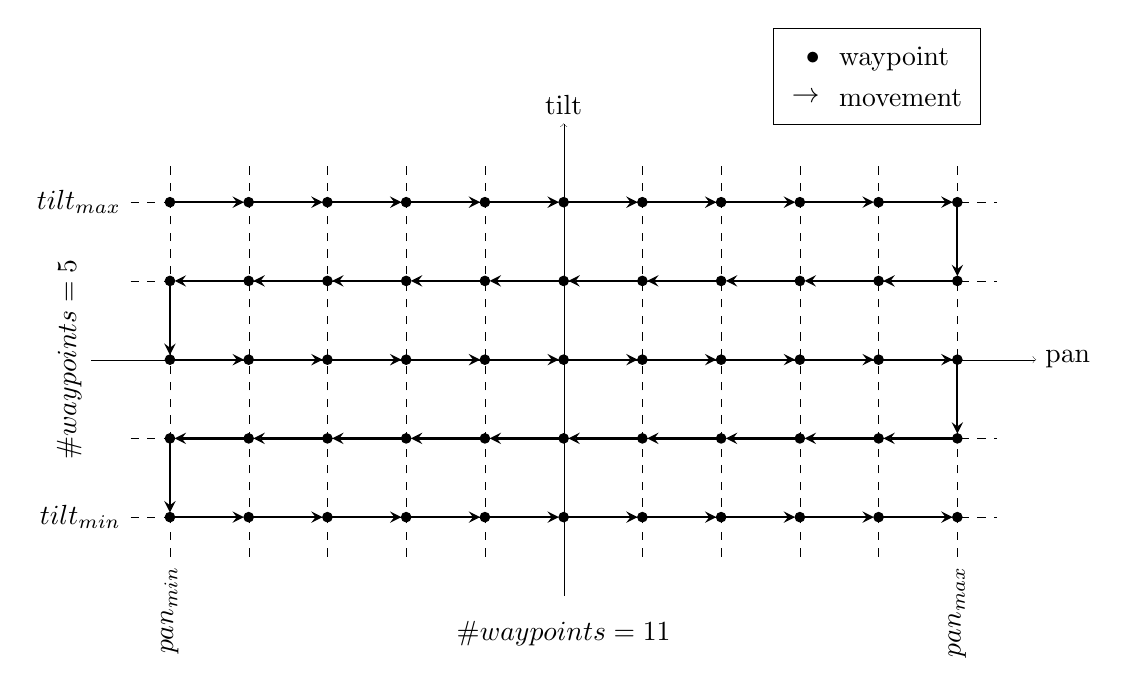
\begin{tikzpicture}

        \draw[->, ultra thin] (-6, 0) -- (6, 0) node[right] {pan};
        \draw[->, ultra thin] (0, -3) -- (0, 3) node[above] {tilt};

        \draw[step=1, ultra thin, dashed] (-5.5, -2.5) grid (5.5, 2.5);

        \foreach \x in {-5,...,5}
            \foreach \y in {-2,...,2}
                \draw[fill=black] (\x, \y) circle (0.06);
        
        \foreach \x in {-5,...,4}
            \foreach \y in {-2,...,2}
                \ifthenelse{\isodd{\y}}{
                    \draw[stealth-, shorten <=0.06cm, thick] (\x, \y) -- (\x+1, \y);  
                }{
                    \draw[-stealth, shorten >=0.06cm, thick] (\x, \y) -- (\x+1, \y);
                };

        \foreach \y in {2,...,-1}
            \ifthenelse{\isodd{\y}}{
                \draw[-stealth, shorten >=0.06cm, thick] (-5, \y) -- (-5, \y - 1);
            }{
                \draw[-stealth, shorten >=0.06cm, thick] (5, \y) -- (5, \y - 1);
            };

        
        \node[anchor=east] at (-5.5, -2) {$tilt_{min}$};
        \node[anchor=east] at (-5.5, 2) {$tilt_{max}$};
        \node[anchor=south, rotate=90] at (-6, 0) {$\#waypoints = 5$};

        \node[anchor=east, rotate=90] at (-5, -2.5) {$pan_{min}$};
        \node[anchor=east, rotate=90] at (5, -2.5) {$pan_{max}$};
        \node[anchor=north] at (0, -3.2) {$\#waypoints=11$};
            
        \matrix[draw, above left, xshift=-1.5cm, yshift=-0.5cm] at (current bounding box.north east) {
            \node[label=right:waypoint] {$\bullet$}; \\
            \node[label=right:movement] {$\rightarrow$}; \\
        };

    \end{tikzpicture}

    \caption{Waypoints and movements in the pan/tilt joint space.}

\label{figure:joint-movement}
\end{figure}


\subsection{Parameterization Considerations}

This methodology has the numerous implications. First, the pan and tilt range is only limited by the PTU capabilities, but it beneficial to use the maximum range possible, in order to get as much data as possible. In this work, most data collected is redundant, for example if multiple tilt angles are used, however this improves the final reconstruction by increasing the density of the point cloud.

Second, the number of laser scans recorded is going to depend on the pan speed and the frequency of scanning of the 2D laser scanner. So, it is expected that a laser scanner with a lower scanning frequency to require a slower speed compared to a faster one, to collect the collect the same amount of data. 
                        
Third, the camera used in this work did not have stabilization so, to get sharp images, a complete immobilization was required in each waypoint. This was achieved by setting a time between the stop of all joints and the capture of the image by the camera. In this work, a time of \SI{1.5}{\second} was enough.
                        
Last, the waypoints' angle increment has to be enough so that part of the previous image appear in the next image, so that every observable part of the scene is seen at least once. This depends heavily on the focal point of the camera: the bigger the focal point, the least area it captures and more waypoints are required.

\subsection{Acquisition node}
\label{section:acquisition-node}


To implement this functionality, a ROS node was developed according to the previously defined specifications. This node, called \emph{single\_acquisition\_node} is present in the \emph{lemonbot\_acquisition} package and the way it is implemented is the following: the PTU movement is controlled by it and the selected messages are republished into a new topic. For convenience, all the acquisition topics are republished into the \emph{/acquisition} namespace. So, during an acquisition, two topics can be found, each one corresponding to each sensor, inside this namespace: the laser scans are in \emph{/acquisition/laserscans} and the images are in \emph{/acquisition/images}. This idea of republishing all the important messages greatly improved the acquisition organization, so all the topics that were required were also republished into this namespace. This topics were the \emph{/acquisition/camera\_info}, containing the intrinsic parameters of the camera, and \emph{/acquisition/tf} and \emph{/acquisition/tf\_static}, containing all the transformations of the robot.

Now, data from these topics need to be saved permanently, so this was done using a ROS tool called \emph{rosbag}, that saves all the data from a predefined set of topics into a binary file called a \emph{bag} file. This was a easy and powerful solution, because it allows the acquisition to be reproduced again, by republishing all the messages back into the system. To save a set of topics, a node called \emph{record} from the \emph{rosbag} package is run with the list of topics that required to be recorded into disk. In this case, the required topics are all the topics inside the \emph{/acquisition} namespace.

To streamline the acquisition process, all these components (the acquisition node, the topic republisher nodes and the rosbag record node) can be all launched through a \emph{launch file}. A set of all the parameters required for each acquisition can be override over the default parameters. Therefore, running an acquisition just requires a single command:

\begin{verbatim}
roslaunch lemonbot_acquisition single_acquisition.launch \
    pan_min:=-90 pan_max:=90 pan_vel:=10 pan_nsteps:=25 \
    tilt_min:=-15 tilt_max:=15 tilt_nsteps:=5
\end{verbatim}

In conclusion, running the previous command will run an acquisition and in the end, a bag file will be present, with the topics \emph{images}, \emph{laserscan}, \emph{camera\_info}, \emph{tf} and \emph{tf\_static}, therefore all the information relevant for the reconstruction.

To have a better insight in the bag file, a tool called \emph{rosbag info} can be used. All the details about when the calibration took place, how long it took as well as how many messages it contains are printed. An example of this information is:

\begin{figure}
    
    \begin{Verbatim}[frame=single, fontsize=\small]
path:        acquisition_2018-09-07-16-01-46.bag
version:     2.0
duration:    4:53s (293s)
start:       Sep 07 2018 16:01:47.11 (1536332507.11)
end:         Sep 07 2018 16:06:40.96 (1536332800.96)
size:        87.0 MB
messages:    6690
compression: none [16/16 chunks]
types:       sensor_msgs/CameraInfo [c9a58c1b0b154e0e6da7578cb991d214]
                sensor_msgs/Image      [060021388200f6f0f447d0fcd9c64743]
                sensor_msgs/LaserScan  [90c7ef2dc6895d81024acba2ac42f369]
                tf2_msgs/TFMessage     [94810edda583a504dfda3829e70d7eec]
topics:      camera_info    953 msgs    : sensor_msgs/CameraInfo
                images          10 msgs    : sensor_msgs/Image     
                laserscan     2788 msgs    : sensor_msgs/LaserScan 
                tf            2938 msgs    : tf2_msgs/TFMessage    
                tf_static        1 msg     : tf2_msgs/TFMessage
    \end{Verbatim}

    \caption{Example of a recorded bag file info}
    \label{figure:bag-file-example}
\end{figure}

\subsection{Data Serialization}
 
Despite their potential, bag files are not the best way to store the acquisition data for the reconstruction pipeline. There are some limitations of bag files in this application. The most noticeable is that the full transformation graph is stored, while in fact only the transformations between the start and end frame of the PTU are needed, as well as the transformations between the PTU mount link and each one of the sensors, which are static. Also, this transformation messages are not synchronized with the laser scans and image messages, which means an interpolation has to be performed each time the data is read. Another drawback is that bag files stores messages in it's own format, which hinder reading and inspecting the data with external tools, which can be helpful to check if an acquisition was successful. For example, the images are serialized into a ROS message, instead of being in a file with a known format, like \emph{JPG}, which would allow for easier access and inspection.

To solve these issues, a preprocessing of the bag files was performed, to convert and extract all the important information into well known and useful formats. Each laser scan was stored in a \emph{AVRO} file row that contains the timestamp (when it was taken), the minimum and maximum angle (aperture of the laser scan), the minimum and maximum ranges that the laser can capture, the transformation of the ptu and the list of all the measured ranges. An example of such row is show in \cref{figure:laserscan-row}, obtained using the \emph{avro cat} command. Each image was stored in a separate \emph{JPEG} file and it's timestamp and transformation was stored in a row, again in a \emph{AVRO} file. The parameters inherent to the acquisition, such as the name of the bag, the extrinsic and intrinsic calibration of the camera used and the extrinsic calibration of the laser was stored in a \emph{YAML} file. The transformations in both the images and laser scans are stored as vector for translation and quaternion for rotation.

\begin{figure}
    
    \begin{Verbatim}[frame=single, fontsize=\small]
{
    "ranges" : [ ... ],
    "limits" : {
        "min" : 0.100000001490116,
        "max" : 29
    },
    "timestamp" : 1536174204611117487,
    "angles" : {
        "min" : -2.35619449615479,
        "max" : 2.35619449615479
    },
    "transform" : {
        "rotation" : [ ... ],
        "translation" : [ ... ]
    }
}
    \end{Verbatim}

    \caption{Example of laser scan row}
\label{figure:laserscan-row}
\end{figure}

\begin{figure}

    \begin{Verbatim}[frame=single, fontsize=\small]
bag: acquisition_2018-09-05-20-02-46.bag
camera:
    extrinsic:
    translation: [ ... ]
    rotation: [ ... ]
    intrinsic:
    principal_point: [ ... ]
    height: 1448
    focal_lenghts: [ ... ]
    width: 1928
    distortion_coef: [ ... ]
    distortion_model: plumb_bob
laser:
    extrinsic:
    translation: [ ... ]
    rotation: [ ... ]
    limits:
        max: 29
        min: 0.1
    angles:
        max: 2.356194
        min: -2.356194
    \end{Verbatim}

    \caption{Example of the parameters YAML file}

\end{figure}



\section{Capture}
\label{section:capture}

As seen before, acquisitions only capture a subset of the scene geometry and color, so multiple acquisitions are required. This problem can be partially solved by recording multiple acquisitions instead of once. Therefore, a capture is a collection of acquisitions of the same scene and it's goal is to contain data from all the scene, in order to create a proper reconstruction of the scene. However, this raises some challenges, on how to plan and execute the multitude of acquisitions and how to merge the data from all of the acquisitions.

\begin{figure}
    
    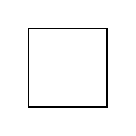
\begin{tikzpicture}
        
        \draw (0,0) rectangle (1, 1);

    \end{tikzpicture}

    \caption{Different positions of the 3D scanner affect the acquisition result}

    \label{figure:scene-acquisitions-example}

\end{figure}


% \chapter{Methodology for Geometry Reconstruction}


\begin{figure}
    
    \centering
    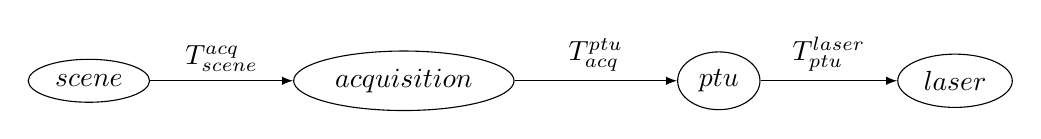
\begin{tikzpicture}
        \node[draw, ellipse] (scene) {$scene$};
        \node[draw, ellipse, right of=scene, xshift=3cm] (acquisition) {$acquisition$};
        \node[draw, ellipse, right of=acquisition, xshift=3cm] (ptu) {$ptu$};
        \node[draw, ellipse, right of=ptu, xshift=2cm] (laser) {$laser$};
        
        \draw[-latex] (scene) -- (acquisition)
        node[midway, above] {$T_{scene}^{acq}$};
        \draw[-latex] (acquisition) -- (ptu)
        node[midway, above] {$T_{acq}^{ptu}$};
        \draw[-latex] (ptu) -- (laser)
        node[midway, above] {$T_{ptu}^{laser}$};
    \end{tikzpicture}
    
    \caption{Transformation graph}
    \label{figure:geometric-transformation-graph}
\end{figure}

\section{Point Registration}
\label{section:point-registration}

Each laser scan is a collection of points in polar coordinates, so each range point $(r_i, \theta_i)$ is transformed to a point in the laser frame of reference according to \cref{eqn:range-to-point}. The angles are uniform distributed between a minimum and maximum angle, $\theta_{min}$ and $\theta_{max}$, respectively, so $\theta_i = \{\theta_{min}, \ \dots, \ \theta_{max}\}, i=1 \dots N$. The index $i$ is defined as the range index of each laser scan.

\begin{equation}\label{eqn:range-to-point}
    \left(
        \begin{array}{c}
            x_i \\
            y_i \\
            z_i \\
        \end{array}
    \right)
    =
    \left(
        \begin{array}{c}
            r_i \cos(\theta_i) \\
            r_i \sin(\theta_i) \\
            0 \\
        \end{array}    
    \right)
\end{equation}

Further on, each point is registered in the referencial of the acquisition. According to the transformation graph (see \cref{figure:geometric-transformation-graph}), there are two transformation from the acquisition frame and the laser scanner frame: the transform from the acquisition frame to the ptu frame $T_{acq}^{ptu}$, which is dynamic and changes for each laser scan, and the transformation from the ptu frame and the laser scanner frame ($T_{ptu}^{laser}$), which is static. This two transformations can be chained together to obtain the point in the acquisition frame, according to \cref{eqn:point-registration}.


\begin{figure}
    
    \centering
    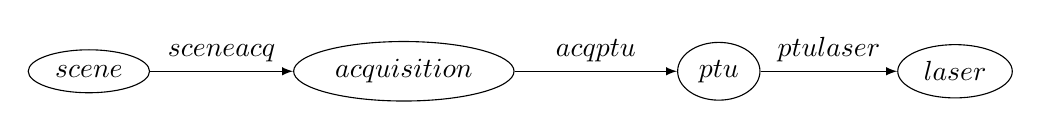
\begin{tikzpicture}
        \node[draw, ellipse] (scene) {$scene$};
        \node[draw, ellipse, right of=scene, xshift=3cm] (acquisition) {$acquisition$};
        \node[draw, ellipse, right of=acquisition, xshift=3cm] (ptu) {$ptu$};
        \node[draw, ellipse, right of=ptu, xshift=2cm] (laser) {$laser$};
        
        \draw[-latex] (scene) -- (acquisition)
        node[midway, above] {$\TF{scene}{acq}$};
        \draw[-latex] (acquisition) -- (ptu)
        node[midway, above] {$\TF{acq}{ptu}$};
        \draw[-latex] (ptu) -- (laser)
        node[midway, above] {$\TF{ptu}{laser}$};
    \end{tikzpicture}
    
    \caption{Transformation graph}
    \label{figure:geometric-transformation-graph}
\end{figure}

\begin{equation}\label{eqn:point-registration}
    P_{i,j} = 
    \left(
        \begin{array}{c}
            x_{i,j} \\ y_{i,j} \\ z_{i,j} \\ 1 \\
        \end{array}    
    \right)
    =
    \TF{acq}{ptu}
    \cdot \TF{ptu}{laser}
    \cdot
    \left(
        \begin{array}{c}
            r_i \cos(\theta_i) \\
            r_i \sin(\theta_i) \\
            0 \\
            1 \\
        \end{array}    
    \right)
\end{equation}

At this phase, each point has 2 indexes, one for the laser scan index $j=1\dots L$ and another for the range index $i=1\dots N$, relative to the each laser scan. Despite that point clouds commonly only one index, at this stage the points are structured in a bidimensional structure of $L \times N$ points. This structure is useful in the normal estimation phase, explained in \cref{section:normal-estimation}.

This reconstruction phase depends heavily on the transformation from the PTU to the laser scanner. This transformation is obtained by a calibration process and is commonly referred as the extrinsic calibration of the laser scanner. The calibration method used to obtain this extrinsic calibration is explained in detain in \cref{section:laser-extrinsic-calibration}.

In conclusion, for each acquisition results a point cloud with $L \times N$ points, where $L$ are the number of laser scans and $N$ the number of range values in each laser scan. Each point can be indexes in a bidimensional index, which can be useful for subsequent algorithms.

\section{Laser Extrinsic Calibration}
\label{section:laser-extrinsic-calibration}

\subsection{Radlocc Method}

\subsection{Proposed Method}

\subsubsection{Paramerization}

\subsubsection{Plane Segmentation}

\subsubsection{Plane Fitting and RMS error}

\subsubsection{Loss Function}
\subsubsection{Optimizer}

\subsubsection{Overview}


\section{Normal Estimation}
\label{section:normal-estimation}

As part of the reconstruction work, it is common to create a mesh using the point cloud, through a process called triangulation. Despite that in this work, this was not performed, it can be done in posterior work. Surface normals are a important property of geometric surfaces and are a requirement for most triangulation algorithms. Also, normals are required for lightning calculation, which can improve the rendering of a point cloud model\footnote{See "Estimating Surface Normals in a PointCloud" in \url{http://pointclouds.org/documentation/tutorials/normal_estimation.php}.}. As an example, the Stanford Bunny model\footnote{From \url{https://www.cc.gatech.edu/~turk/bunny/bunny.html}.} rendered with and without lightning are show in \cref{figure:bunny-normals}. As can be seen, lightning can improve the perception of the geometry of the point cloud model.

Normal estimation is quite trivial for surfaces, but for point clouds the process is quite not as easy. Usually there are two ways to estimate the normals: either by meshing the surface first, and then calculate the normals for the mesh, or using the point cloud itself to infer the normals. However, most meshing algorithms already require the normals to achieve a good result, so the latter option is more effective.

\begin{figure}[h]
    
    \centering
    \begin{subfigure}{0.4\textwidth}
        \centering
        \includegraphics[height=6cm]{bunny-with-normals}     
    \end{subfigure}%
    \begin{subfigure}{0.4\textwidth}
        \centering
        \includegraphics[height=6cm]{bunny-without-normals}     
    \end{subfigure}

    \caption{Stanford rabbit rendering with lightning (on the left), using the normals information, and without lightning (on the right).}
    \label{figure:bunny-normals}

\end{figure}

The most common solution is, for each point, to find the $k$ closest points, defined as the $k$-neighborhood of a point, and calculate the normal of the best-fitting plane formed by this points. However, finding the $k$-neighborhood of all the points in a point cloud has a time complexity $O(N \log N)$, so it can become quite slow for point clouds with a large number of points. In this work, an alternative solution was used to find the closest points, exploiting the bidimensional structure of the point cloud. This solution has a linear time complexity $O(N)$, which makes it a valuable solution for large point clouds.

The solution uses the fact that each point in the point cloud resulting from \cref{section:point-registration} has two indexes, one for the range index $i$ and one for the laser scan $j$. For each laser scan, each point $p_i$ has a neighborhood ${p_{i-k}, \ \dots, \ p_{i+k}}$, because each subsequent point has an increasing angle to the previous point. Between successive laser scans each point has an increasing angle (the pan angle) to the previous one. Therefore, for this algorithm, the neighborhood of each point: 

\begin{equation}
\label{eqn:point-neighborhood}
    neighborhood(p_{i,j}, k_1, k_2) = \{p_{i-k_1, j-k_2}, \ \dots, \ p_{i+k_1, j+k_2}\}.
\end{equation}

\noindent
The value of $k_1$ and $k_2$ have to be adjusted for a better result, because if the values are large, fine details are going to disappear and edges are going to be smeared, and on the other hand if the values are small, the surface will appear as too noisy. In this work, the value of $k_1$ and $k_2$ was 3, so the neighbor has 9 points.

Then, for each point, the tangent plane that fits the neighborhood is calculated, which in turn is a least-square plane fitting problem. This is usually solved by an analysis of Principal Component Analysis, as explained in \cref{section:calibration-cost-function}. This method will compute the direction of the normal $n$ for each point.

Then, the orientation of the point has to be defined, because the result of the PCA is ambiguous, which may lead to inconsistent normals in the point cloud. In this case, the solution found was to orientate the normals towards the frame of the 3D scanner, which for each acquisition in the origin of the coordinate system. Therefore, each normal has to satisfy:

\begin{equation}
\label{eqn:normal-orientation}
    n \cdot p < 0.
\end{equation}

\section{Acquisition Registration}
\label{section:acquisition-registration}

During an acquisition multiple acquisitions are done and to each one corresponds a transformation (position and orientation) to the scene referencial. In this section, a method is described to find each one of this transformations, so all the acquisitions are merged into a single point cloud. The method chosen is the ICP or Iterative Closest Point. This method is capable of aligning two point clouds, the reference and the target point cloud, by finding the transformation between the second to the first one. This is also known as point cloud registration.

\subsection{ICP}

\newcommand{\T}{\mathcal{T}}
\newcommand{\Pt}{\mathcal{P}}
\newcommand{\Q}{\mathcal{Q}}

This method can formally be described as follows: let $\Pt$ be the target point cloud and $\Q$ the reference point cloud. Then, the aim of the registration is to estimate the transformation $\T$ from the referencial of $\Pt$ to $\Q$ by minimizing the error function $\textrm{error}(\Pt, \Q)$ in \cref{eqn:icp-transformation-function}, where $\T(\Pt)$ is the result of the application of the transformation $\T$ to the point cloud $\Pt$.

\begin{equation}
\label{eqn:icp-transformation-function}
    \mathcal{T} = \underset{\T}{\textrm{argmin}}(\mathrm{error}(\T(\Pt), \Q))
\end{equation}

The error function $error(P, Q)$ is computed on pair of points that are associated between the two point clouds. This association is, ideally, between points that are closest in position in both point clouds. Then, the distance between the matching points $(p_i, q_i)$ are used in the error function in \cref{eqn:icp-error-function}. The matching algorithm can be based on features or geometric properties, so a better matching can be found. In this work, a simple point-to-point matching.

\begin{equation}
\label{eqn:icp-error-function}
    \textrm{error}(\Pt, \Q) = \sum_{(p_i, q_i)}{|p_i - q_i|}
\end{equation}

In order to make the error function more robust, outlier points can be removed first from the match list. In addition, weights $w_i$ can be associated to each matching points $(p_i, q_i)$ to increase or decrease the influence of each matching points in the error function. As an example, normals can be used as a weight, so points with similar normals ($w_i = n_{p_i} \cdot n_{q_i}$) have a greater influence in the error function. 

However, the result of this minimization is always always dependant on the association between the points, which, unless the descriptors are good enough (like visual correspondences), the matching is not perfect, and is worst the farther apart both point clouds are. The idea behind the ICP algorithm is that, even with a bag association, the resulting estimate can be used to find a better one. So, the ICP algorithm creates a series of transformation $\T_i$ at each iteration, yielding a new transformed point cloud $\Pt_i$. Then, the next transformation is found:

\begin{equation}
    \T_{i+1} = \underset{T}{\textrm{argmin}}(\textrm{error}(\T_i(\Pt_i), \Q))
\end{equation}

Finally, the final transformation estimate is the composition of all the intermediary transformations:

\begin{equation}
    \T = \T_1 \circ \T_2 \circ \dots \circ \T_N
\end{equation}

\subsection{Multiple Point Cloud ICP}
\label{section:multiple-pointcloud-icp}

However, ICP can only register pairs of point clouds, whereas this work requires a registration of $N$ point clouds, corresponding to $n$ acquisitions. So, a technique has to be found so that the ICP algorithm can be used with $n$ point clouds. Three of this such techniques are now describes, ordered by their complexity.

The first approach and the easier one to implement is to register each point clouds sequencially. In other words, this method registers the point cloud $\Pt_i$ to the point cloud $\Pt_{i-1}$ and the transformation $\T_{i-1}^{i}$ is found. The final accumulated point cloud is assembled using the \cref{eqn:registration-simple-method-calculation}. This method is the one that requires less overall registration, but has the downside that the transformation errors increases for each successive point cloud. This approach is shown in \cref{figure:multiple-icp-method-1}.

\begin{equation}
\label{eqn:registration-simple-method-calculation}
    \Pt = \bigcup{\left(\T_1^2 \circ \T_2^3 \circ \dots \circ \T_{i-1}^i\right)(\Pt_i)}
\end{equation}

The next approach is widely used in robotics for Simultaneous Location and Mapping (SLAM). This method holds an accumulated point cloud $A$ in memory, and each new incoming point cloud $\Pt$ registers to the accumulated point cloud and afterwards it is merged into $A$, which is then used for the next iteration, as shown in \cref{figure:multiple-icp-method-2}. It has the advantage that each new registration is done against a wider point cloud and has a smaller influence than in the previous method. Also, at each iteration the current pose of the 3D scanner is obtained, which is used as an initial estimate for the next iteration. However, the accumulated point cloud grows at each iteration, so a down-sampling is done at each iteration to keep the number of points bounded. In conclusion, each iteration can be calculated as:

\begin{align}
    \T_{i} = & \textrm{ICP}(A, \Pt_{i}, \T_0 = \T_{i-1}) \\
    A_{i+1} = & A{i} \bigcup \T_{i}(\Pt_i)
\end{align}

The last approach is the most complex. The idea of this approach is to minimize the number of transformation combinations, to minimize the propagation of the error. In particular, the registrations for the $N$ points clouds are done pairwise and are merged together to create $N/2$ point clouds. Then, this process is done recursively until an unique point cloud is obtained. This way, the maximum number of transformation combinations are equal to the number of levels of the tree, which is $\log_2(N)$, instead of $N$ combinations in the first approach. This algorithm is formalized in \cref{eqn:registration-tree-method-1,eqn:registration-tree-method-2}, for a list of point clouds $S=\left\{P_1, P_2, \ \dots, \ P_n\right\}$. At each level $l$ a new list of point clouds $^{l}P$ and transformations $^{l}T$ are computed, as shown in \cref{figure:multiple-icp-method-3}.

\begin{align}
    ^{l}\T = & \left\{\textrm{ICP}(^{l-1}\Pt_1, ^{l-1}\Pt_2), \ \dots, \ \textrm{ICP}(^{l-1}\Pt_{n-1}, ^{l-1}\Pt_{n}) \right\}
        \label{eqn:registration-tree-method-1} \\
    ^{l}\Pt = & \left\{^{l-1}\Pt_1 \bigcup{^{l}\T_1(^{l-1}\Pt_2}), \ \dots, \ ^{l-1}\Pt_{n-1} \bigcup{^{l}\T_{n/2}(^{l-1}\Pt_n)}\right\}
        \label{eqn:registration-tree-method-2}
\end{align}

In conclusion, three methods are possible to extend the ICP algorithm to multiple point clouds. After all the registrations are performed, point cloud can be assembled from all the point clouds, to form a big point cloud of the final scene. There is, however, a limitation of all this methods, because all of them have the principle that every point cloud is close to the previous one, which can be false. In this work, this was ensured in the capture methodology. 

\begin{figure}
    \centering
    \begin{subfigure}[t]{0.3\textwidth}
        \centering
        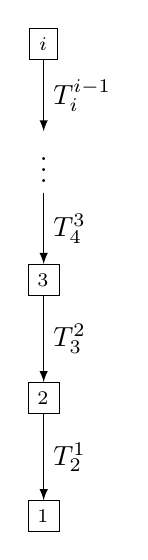
\begin{tikzpicture}
            \node[draw] (P1) at (0,0) {$\Pt_1$};
            \node[draw] (P2) at (0,1.5) {$\Pt_2$};
            \node[draw] (P3) at (0,3) {$\Pt_3$};
            \node (P4) at (0,4.5) {$\vdots$};
            \node[draw] (Pi) at (0,6) {$\Pt_i$};

            \draw[-latex] (P2) -- (P1) node[midway, anchor=west] {$T_2^1$};
            \draw[-latex] (P3) -- (P2) node[midway, anchor=west] {$T_3^2$};
            \draw[-latex] (P4) -- (P3) node[midway, anchor=west] {$T_4^3$};
            \draw[-latex] (Pi) -- (P4) node[midway, anchor=west] {$T_i^{i-1}$};
        \end{tikzpicture}

        \caption{First method}
        \label{figure:multiple-icp-method-1}
    \end{subfigure}%
    \begin{subfigure}[t]{0.3\textwidth}
        
        \centering
        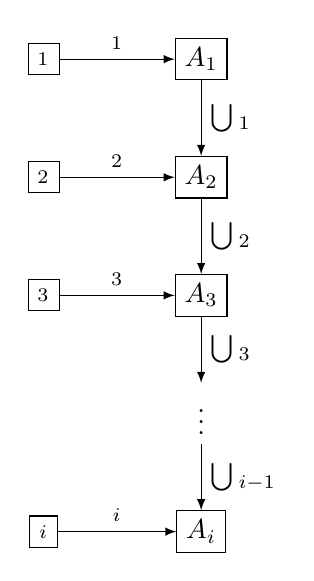
\begin{tikzpicture}
            \node[draw] (A1) at (0,0) {$A_1$};
            \node[draw] (A2) at (0,-1.5) {$A_2$};
            \node[draw] (A3) at (0,-3) {$A_3$};
            \node (A4) at (0,-4.5) {$\vdots$};
            \node[draw] (Ai) at (0,-6) {$A_i$};

            \node[draw, left of=A1, xshift=-1cm] (P1) {$\Pt_1$};
            \draw[-latex] (P1) -- (A1) node[midway, above] {$\T_1$};

            \node[draw, left of=A2, xshift=-1cm] (P2) {$\Pt_2$};
            \draw[-latex] (P2) -- (A2) node[midway, above] {$\T_2$};

            \node[draw, left of=A3, xshift=-1cm] (P3) {$\Pt_3$};
            \draw[-latex] (P3) -- (A3) node[midway, above] {$\T_3$};

            \node[draw, left of=Ai, xshift=-1cm] (Pi) {$\Pt_i$};
            \draw[-latex] (Pi) -- (Ai) node[midway, above] {$\T_i$};

            \draw[-latex] (A1) -- (A2) node[midway, right] {$\bigcup{\Pt_1}$};
            \draw[-latex] (A2) -- (A3) node[midway, right] {$\bigcup{\Pt_2}$};
            \draw[-latex] (A3) -- (A4) node[midway, right] {$\bigcup{\Pt_3}$};
            \draw[-latex] (A4) -- (Ai) node[midway, right] {$\bigcup{\Pt_{i-1}}$};
        \end{tikzpicture}

        \caption{Second method}
        \label{figure:multiple-icp-method-2}
    \end{subfigure}%
    \begin{subfigure}[t]{0.4\textwidth}
        
        \centering
        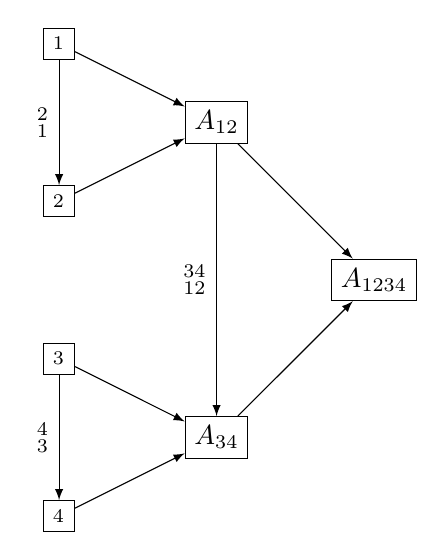
\begin{tikzpicture}
            \node[draw] (P1) at (0,0)  {$\Pt_1$};
            \node[draw] (P2) at (0,-2) {$\Pt_2$};
            \node[draw] (P3) at (0,-4) {$\Pt_3$};
            \node[draw] (P4) at (0,-6) {$\Pt_4$};

            \node[draw] (A12) at (2, -1) {$A_{12}$};
            \node[draw] (A34) at (2, -5) {$A_{34}$};
            \node[draw] (A1234) at (4, -3) {$A_{1234}$};

            \draw[-latex] (P1) -- (A12);
            \draw[-latex] (P2) -- (A12);
            \draw[-latex] (P3) -- (A34);
            \draw[-latex] (P4) -- (A34);
            \draw[-latex] (A12) -- (A1234);
            \draw[-latex] (A34) -- (A1234);

            \draw[-latex] (P1) -- (P2) node[midway, left] {$\T_1^2$};
            \draw[-latex] (P3) -- (P4) node[midway, left] {$\T_3^4$};
            \draw[-latex] (A12) -- (A34) node[midway, left] {$\T_{12}^{34}$};

        \end{tikzpicture}
        \caption{Third method}
        \label{figure:multiple-icp-method-3}
    \end{subfigure}%


    \caption{Multiple Point Cloud ICP approaches}
    \label{figure:registration-methods-approaches}
\end{figure}
\section{Filters}
\label{section:filters}

The final point cloud, after the assembly from every acquisition's point cloud, can have unnecessary or redundant information, which can make the point cloud size too large for any use. A common solution is to use filters to remote unnecessary points and downsample the point cloud.

\subsection{NaN Removal}

The first filter is the Not a Number removal, or NaN removal. In the acquisition, any range that is not measured is stored as a NaN, to signal that they are missing. During the point registration phase, all this missing ranges remain as NaN, and should be removed, because their information is irrelevant and take as much space as a real value. So, each point that contains a NaN value is removed from the final point cloud.

\subsection{Statistic Outlier Removal}

Usually point clouds contains different point densities, dependent on the distance of the object to the sensor. Also, measurement errors also occur next to edges or corners. As a result, point clouds tend to have sparse outliers that can affect subsequent algorithms, like segmentation or registration algorithms. A usual solution is to perform an statistically analysis on each point, removing the ones that do not reach a certain criteria. In particular, the mean distance of each point to its neighbors is computed, and if this distance is outside an interval centered in the mean of all the distances, then it is removed. An example can be seen in \cref{figure:sor-filter}.

\begin{figure}[h]
    
    \centering
    \begin{subfigure}[t]{0.5\textwidth}
        
        \centering
        \includegraphics[width=0.8\textwidth]{table-with-outliers}
        \caption{Before SOR}
        \label{figure:sor-filter-before}
    \end{subfigure}%
    \begin{subfigure}[t]{0.5\textwidth}
        \centering
        \includegraphics[width=0.8\textwidth]{table-without-outliers}
        \caption{After SOR}
        \label{figure:sor-filter-after}
    \end{subfigure}

    \caption{SOR filter in a point cloud}
    \label{figure:sor-filter}
\end{figure}

\subsection{Voxel Grid Downsampling}

This method downsamples, that is, reduce the number of points of a point cloud, using a voxel grid. A voxel is a cubical space and is the element in a tridimensional grid. So, each point in the point cloud belongs to some voxel. Then, in each voxel, all the points are represented by their centroid. This is an effective and fast method to downsample a point cloud. The level of detail can be parameterized with the voxel leaf-size (the size of each voxel in the $x,y,z$ direction). A smaller leaf-size maintains more details but generates a bigger point cloud. A bigger leaf-size does not keep as much detain but generates a smaller point cloud. As an example, \cref{figure:lucy-voxel-grid} shows the Stanford Lucy model \cite{stanford-scanning-rep} after a voxel grid downsampling with different leaf size values: \cref{figure:lucy-voxel-grid-2mm} with \SI{2}{\milli\meter} (288.000~pts), \cref{figure:lucy-voxel-grid-5mm} with \SI{5}{\milli\meter} (55.000~pts) and \cref{figure:lucy-voxel-grid-8mm} with \SI{2}{\milli\meter} (18.000~pts).

\begin{figure}[h]
    
    \centering
    \begin{subfigure}[t]{0.3\textwidth}
        \centering
        \includegraphics[height=6cm]{lady-voxel-2mm}
        \caption{Leaf size of \SI{2}{\milli\meter}}
        \label{figure:lucy-voxel-grid-2mm}
    \end{subfigure}%
    \begin{subfigure}[t]{0.3\textwidth}
        \centering
        \includegraphics[height=6cm]{lady-voxel-5mm}
        \caption{Leaf size of \SI{5}{\milli\meter}}
        \label{figure:lucy-voxel-grid-5mm}
    \end{subfigure}%
    \begin{subfigure}[t]{0.3\textwidth}
        \centering
        \includegraphics[height=6cm]{lady-voxel-8mm}
        \caption{Leaf size of \SI{8}{\milli\meter}}
        \label{figure:lucy-voxel-grid-8mm}
    \end{subfigure}

    \caption{Stanford Lucy scan \cite{stanford-scanning-rep} after a voxel grid downsampling with different leaf sizes}
    \label{figure:lucy-voxel-grid}
\end{figure}

% \chapter{Methodology for Image Registration}
\label{section:methodology-for-image-registration}

This chapter describes the methodology for image registration, that is, the process that colorizes (defines the color) the point cloud based on the images taken in the acquisitions. This method can be split into two parts: the Color Registration (\cref{section:color-registration}), where the process is described per-image and each image colorizes a portion of the point cloud, and the Color Fusion (\cref{section:color-fusion}), where all the colorized point cloud partials are merged into the final colorized point cloud. Also, the pixel registration relies on a camera calibration, both the intrinsic calibration and also the extrinsic, so two methods are shown to obtain this calibration (\cref{section:camera-intrinsic-calibration,section:camera-extrinsic-calibration}).

\section{Color Registration}
\label{section:color-registration}

This method describes how to colorize a point cloud based on a single image, using a working principle similar to the ray tracing used in computer graphics. As an overview, each point in the point cloud can be transformed as a ray in the camera perspective, which is basically the path from the eye point to the point. This ray can be used to retrieve the original color of the point from the image. However, this process is not so straightforward, because the position and orientation of the camera has to be very precise and occluded points need to be rejected.

\subsection{Point to pixel coordinates transformation}

To start, each point has to be transformed, because the original point is registered in the scene coordinate frame ($p_{scene}$) and has to be registered into the camera coordinate frame ($p_{camera}$). So, the transformations $\prescript{acquisition}{scene}{\mathcal{T}}$, $\prescript{ptu}{acquisition}{\mathcal{T}}$, $\prescript{camera}{ptu}{\mathcal{T}}$ can be used according to \cref{eqn:point-camera-transformation}. The $\prescript{acquisition}{scene}{\mathcal{T}}$ transformation is obtained in \cref{section:acquisition-registration}, $\prescript{ptu}{acquisition}{\mathcal{T}}$ is the transformation of the PTU and $\prescript{camera}{ptu}{\mathcal{T}}$ is the extrinsic calibration of the camera and the method to obtain it is in \cref{section:camera-extrinsic-calibration}. The transformation graph can be seen in \cref{fig:color-registration-3d}.

\begin{equation}
    \label{eqn:point-camera-transformation}
    p_{scene} =
        \prescript{acquisition}{scene}{\mathcal{T}} \cdot 
        \prescript{ptu}{acquisition}{\mathcal{T}} \cdot
        \prescript{camera}{ptu}{\mathcal{T}} \cdot p_{camera}
\end{equation}

\begin{figure}
    \tdplotsetmaincoords{70}{150}
    \centering
    \begin{tikzpicture}[tdplot_main_coords]

        \coordinate (scene) at (-4,0,0);
        \coordinate (acquisition) at (7, 5, 5);
        \coordinate (ptu) at (10, 5, 7);
        \coordinate (camera) at (8, 7, 10);

        \tikzset{
            axes/.pic = {
                \draw[thick,->] (0,0,0) -- +(-1,0,0) node[anchor=west]{$y$};
                \draw[thick,->] (0,0,0) -- +(0,1,0) node[anchor=west]{$x$};
                \draw[thick,->] (0,0,0) -- +(0,0,1) node[anchor=south]{$z$};
            }
        };

        \newcommand{\axes}[1] {
            \draw[thick,->] #1 -- +(-1,0,0) node[anchor=west]{$y$};
            \draw[thick,->] #1 -- +(0,1,0) node[anchor=north west]{$x$};
            \draw[thick,->] #1 -- +(0,0,1) node[anchor=south]{$z$};
        }

        \draw pic at (scene) {axes};
        \node[below left, scale=0.7] at (scene) {scene};

        \draw pic at (acquisition) {axes};
        \node[below left, scale=0.7] at (acquisition) {acquisition};

        \tdplotsetrotatedcoords{0}{0}{30}
        \draw[tdplot_rotated_coords] pic at (ptu) {axes};
        \node[below left, scale=0.7] at (ptu) {ptu};

        \tdplotsetrotatedcoords{10}{-85}{0}
        \draw[tdplot_rotated_coords] pic at (camera) {axes};
        \node[above left, scale=0.7] at (camera) {camera};

        \path[-latex]
            (scene) edge[bend right=10] node[midway, above] {$\prescript{acquisition}{scene}{\mathcal{T}}$} (acquisition)
            (acquisition) edge[bend left=20] node[midway, below left] {$\prescript{ptu}{acquisition}{\mathcal{T}}$} (ptu)
            (ptu) edge[bend left=20] node[midway, above left] {$\prescript{camera}{ptu}{\mathcal{T}}$} (camera);

        \draw[tdplot_rotated_coords]
            ($(camera) + ( 0.8, 1, 3)$) -- 
            ($(camera) + ( 0.8,-1, 3)$) -- 
            ($(camera) + (-0.8,-1, 3)$) --
            ($(camera) + (-0.8, 1, 3)$) -- cycle;
        \draw[tdplot_rotated_coords, -latex, thick]
            ($(camera) + ( 0.8, -1, 3)$) -- +(0, 2.5, 0)
            node[above] {$u$};
            \draw[tdplot_rotated_coords, -latex, thick]
            ($(camera) + ( 0.8, -1, 3)$) -- +(-2, 0, 0)
            node[below] {$v$};
        
        \coordinate (point) at (0, 6, 10);
        
        \coordinate (projected) at ($0.35*(point)+{1-0.35}*(camera)$);
        \node[tdplot_rotated_coords, scale=2]
            at (projected)
            {$.$};
        \node[tdplot_rotated_coords, scale=0.6, above]
            at (projected)
            {$(u_i,v_i)$};

        \node[scale=2] at (point) {$.$};
        \node[above right] at (point) {$p_i$};

        \draw[-latex] (camera) -- (point);

        
    \end{tikzpicture}

    \caption{Color registration for a single point}
    \label{fig:color-registration-3d}
\end{figure}

Next, each point was transformed into pixel coordinates $(u, v)$, using the pinhole camera model. This model defined how a light ray in projected in the image sensor of a camera and has two parameters: the focal length $f = (f_x, f_y)$ and optical center $(c = (c_x, c_y))$. This parameters are obtained in the intrinsic calibration of the camera (\cref{section:camera-intrinsic-calibration}). According to this model, each point is projected as pixel coordinates $(u, v)$ to a plane located a unit distance from the camera eye point, using the perspective projection matrix in \cref{eqn:perspective-matrix}, according to:

\begin{equation}
    \label{eqn:perspective-matrix}
    \mathcal{P} =
    \left[
        \begin{array}{ccc}
            f_x & 0   & c_x \\
            0   & f_y & c_y \\
            0   & 0   & 1   \\
        \end{array}    
    \right],
\end{equation}

\begin{equation}
    \label{eqn:perpective-transformation}
    \left(
        \begin{array}{c}
            u z \\ v z \\ z \\
        \end{array}    
    \right)
    =
    \mathcal{P} \cdot
    \left(
        \begin{array}{c}
            x \\ y \\ z \\
        \end{array}    
    \right).
\end{equation}

\subsection{Camera Distortion}

The pinhole camera model does not regard the distortion caused by the lens, which is not negligible for most cameras. The two sources of distortion are radial and tangential distortion. Radial distortion makes straight lines appear curved, known as the barrel distortion and pincushion distortion. This distortion is highly noticed in images taken with fish-eye lenses, as seen in \cref{fig:fisheye}. This distortion can be solved by transforming the $(u, v)$ with \cref{eqn:radial-distortion}. Similarly, tangential distortion is caused by a misalignment of the lens to the imaging plane, which causes areas in the image to appear closer than expected. This deformation can be solved with the \cref{eqn:tangential-distortion}. In brief, to undistort the image five parameters need to be determined, also known as the distortion coefficients: $\{k_1, k_2, p_1, p_2, k_3\}$, which are obtained in the camera intrinsic calibration method, described in \cref{section:camera-intrinsic-calibration}.

\begin{align}
    \label{eqn:radial-distortion}
    \left(
        \begin{array}{c}
            u \\ v \\
        \end{array}
    \right)_{calibrated}
    & =
    (1 + k_1 r^2 + k_2 r^4 + k_3 r^6)
    \left(
        \begin{array}{c}
            u \\ v \\
        \end{array}
    \right).
    \\
    \label{eqn:tangential-distortion}
    \left(
        \begin{array}{c}
            u \\ v \\
        \end{array}
    \right)_{calibrated}
    & =
    \left(
        \begin{array}{c}
            u \\ v \\
        \end{array}
    \right)
    + 
    \left(
        \begin{array}{c}
            2 p_1 u v + p_2 (r^2 + 2u^2) \\
            p_2 (r^2 + 2v^2) + 2 p_2 u v \\
        \end{array}
    \right).
\end{align}

\begin{figure}[h]
    
    \centering
    \includegraphics[width=0.65\textwidth]{fisheye}

    \caption{Barrel distortion in fish eye lens.}
    \label{fig:fisheye}

\end{figure}

\subsection{Point filtering}

Not all points are eligible for the color registration, based on it's location and camera properties, so two filtering steps were used: the first filter removes the points outside the view frustum and the second removes the hidden points.

\subsubsection{View Frustrum Removal Filter}

The view frustum is defined as the region of space that is captured by the camera sensor, which for pinhole cameras is a pyramid truncated by two parallel planes (the near and far clipping planes), as seen in \cref{fig:visual-frustrum-3d}. The sides of the frustum are limited by the size of the sensor, so the points that lie outside the bounding box defined by the points $(0,0)$ and $(width, height)$ is excluded.


\begin{figure}[h]
    
    \tdplotsetmaincoords{70}{140}
    \centering
    \begin{tikzpicture}[tdplot_main_coords]
        \coordinate (eye) at (0,0,0);

        \node[above left, scale=0.7] at (eye) {eye point};

        \draw[thick,->] (eye) -- +(-10,0,0) node[anchor=north west]{$z$};
        \draw[thick,->] (eye) -- +(0,1,0) node[anchor=north west]{$x$};
        \draw[thick,->] (eye) -- +(0,0,-1) node[anchor=north]{$y$};

        \newcommand{\drawfrustumlines}[2]{
            \def\x{#1/#2};
            \draw[dashed] (eye) -- (#1, \x, \x);
            \draw[dashed] (eye) -- (#1, -\x, \x);
            \draw[dashed] (eye) -- (#1, \x, -\x);
            \draw[dashed] (eye) -- (#1, -\x, -\x);
        }
        \newcommand{\drawfrustum}[3]{
            \def\a{#1/#3};
            \def\b{#2/#3};
            \draw (#1, \a, \a) -- (#1, -\a, \a) -- (#1, -\a, -\a) -- (#1, \a, -\a) --cycle;
            \draw (#2, \b, \b) -- (#2, -\b, \b) -- (#2, -\b, -\b) -- (#2, \b, -\b) --cycle;
            \draw (#1, \a, \a) -- (#2, \b, \b);
            \draw (#1, -\a, \a) -- (#2, -\b, \b);
            \draw (#1, -\a, -\a) -- (#2, -\b, -\b);
            \draw (#1, \a, -\a) -- (#2, \b, -\b);

        }

        \drawfrustumlines{-10}{8};
        \drawfrustum{-8}{-4}{8};

        \draw[dashed] (0,0,-1.5) -- (0,0, -2);
        \draw[dashed] (-4,0,-2) -- (-4, 0, -1);
        \draw[dashed] (-8,0,-2) -- (-8, 0, -1.5);

        \draw[latex-latex] (0,0,-2) -- (-4, 0, -2) node[above, midway, sloped] {$z_{near}$};
        \draw[-latex] (-4,0,-2) -- (-8, 0, -2) node[above, midway, sloped] {$z_{far}$};
        
    \end{tikzpicture}

    \caption{Representation of the visual frustum of the camera}
    \label{fig:visual-frustrum-3d}

\end{figure}

The near and far clipping planes should reject the points based on the depth of field of the camera. The depth of field, or DOF, is the distance from the camera to the objects range, so that this objects are in focus. If the object falls out of this range, it starts to loose focus incrementally the farther out it is. There is a point where the object is sharper, which is called point of optimal focus. Two factor influences the DOP: the aperture size and the focal length. The aperture influences the amplitude of the DOF, so a bigger aperture results in a narrower DOF, and the focal length defines the point of optimal focus, so a bigger focal length moves the DOF farther away from the camera. The near and far clipping plane should defined to be the boundaries of the DOF, so that all points are in focus.

Based on the frustum of the camera defined above, the points that do not respect \cref{eqn:frustum-condition} should be rejected.

\begin{equation}
    \label{eqn:frustum-condition}
    \begin{aligned}
                 & 0        & < u & < width \\
        \wedge \ & 0        & < v & < height \\
        \wedge \ & z_{near} & < z & < z_{far} \\
    \end{aligned}
\end{equation}

\subsubsection{Hidden Point Removal Filter}

Not all points that lie on the frustum of the camera are seen by the camera, because some of this points are occluded by nearer objects, so they need to be removed. A fast and straightforward solution is to use the point cloud resulting from the same acquisition as the image, because the sensor are considered close together. However, this is not the best solution, as it would be better if the point cloud obtained after the acquisition registration was used.

In \cite{katz07}, an simple and fast operator, the Hidden Point Removal, or HPR, determines the visibility of point sets, viewed from a given viewport. This method is easily implemented and has a asymptotic complexity of $O(n \log n)$, where $n$ is the number of points in the point cloud. Moreover, this method works well for both sparse and dense point clouds.

The HPR operator operates on a set of points $\mathcal{P} = \{p_i | i = 1 \dots n \}$, and the goal is to determine whether $p_i$ is visible from a viewpoint $\mathcal{C}$. In this application, $C$ is the origin of the point cloud. The algorithm consists of two steps: the inversion and the construction of the convex hull.

The inversion step maps each point $p_i$ along the ray from $\mathcal{C}$ to $p_i$, such that $|p_i|$ is monotonically decreasing. There are multiple ways to perform the inversion, but in \cite{katz07} the \emph{spherical flipping} was used. Spherical flipping reflects a point $p_i$ with respect to a sphere of radius $R$ to the new point $\hat{p_i}$ by applying:

\begin{equation}
    \label{eqn:spherical-flipping}
    \hat{p_i} = p_i + 2 (R - |p_i|) \frac{p_i}{|p_i|}.
\end{equation}

Afterwards, the convex hull of $\hat{\mathcal{P}} \bigcup \{\mathcal{C}\}$, where $\hat{\mathcal{P}}$ is the transformed point set and $\mathcal{C}$ is the center of the sphere, is computed. Finally, the points that lie in the convex hull are the visible points of the point set.

This algorithm only has a parameter, which is the radius $R$ of the sphere used for the spherical flipping, which influences the amount of false positives of the algorithm. In general, $R$ is determined based on the maximum point length $max(|p_i|)$ and a exponential factor $\alpha$, such that $R = max(|p_i|) \times 10^{\alpha}$. In this application, a factor of $\alpha = 3$ was adequate.

As an example, the HPR operator was used in the Stanford Bunny\footnote{From https://www.cc.gatech.edu/~turk/bunny/bunny.html.} point cloud, as seen in \cref{fig:hpr-operator-bunny} and, as seen, \cref{fig:after-hpr} only presents the points that are visible, as opposed to \cref{fig:before-hpr}.

\begin{figure}[h]
    
    \centering
    \begin{subfigure}{0.5\textwidth}
        \centering
        \includegraphics[height=6cm]{bunny-before-hpr}
        \caption{Before the HPR}
        \label{fig:before-hpr}
    \end{subfigure}%
    \begin{subfigure}{0.5\textwidth}
        \centering
        \includegraphics[height=6cm]{bunny-after-hpr}
        \caption{After the HPR}
        \label{fig:after-hpr}
    \end{subfigure}

    \caption{Result of the HPR operator in the Bunny point cloud}
    \label{fig:hpr-operator-bunny}

\end{figure}

\subsection{Color Attribution}

\newcommand\ceil[1]{\lceil #1 \rceil}
\newcommand\floor[1]{\lfloor #1 \rfloor}

Finally, the color is extracted from the image at the pixel coordinates $(u, v)$ and saved for the correspondent pixel. Because images are discrete, the color is interpolated using a bilinear interpolation, which uses the neighbor pixels to interpolate the color $C$ at $(u, v)$ in an image $I$ according to \cref{eqn:bilinear-interpolation} (the ceil and floor operators are, respectively, $\ceil{\cdot}$ and $\floor{\cdot}$). The interpolation can be visualized in \cref{fig:bilinear-interpolation}.

\begin{equation}
    \label{eqn:bilinear-interpolation}
    \begin{aligned}
        C(u, v) = \ & (u - \ceil{u}) \ (v - \ceil{v}) \ I_{\floor{u}, \floor{v}} \\
                + \ &  (u - \ceil{u}) \ (v - \floor{v}) \ I_{\floor{u}, \ceil{v}} \\
                + \ &  (u - \floor{u}) \ (v - \ceil{v}) \ I_{\ceil{u}, \floor{v}} \\
                + \ &  (u - \floor{u}) \ (v - \floor{v}) \ I_{\ceil{u}, \ceil{v}} \\
    \end{aligned}
\end{equation}

\begin{figure}[h]
    \centering
    \begin{tikzpicture}
        \draw[-latex] (-1, -1) -- (4, -1) node[below] {$u$};
        \draw[-latex] (-1, -1) -- (-1, 4) node[left] {$v$};

        \coordinate (c00) at (0,0);
        \coordinate (c10) at (3,0);
        \coordinate (c01) at (0,3);
        \coordinate (c11) at (3,3);
        \coordinate (c) at (1.7, 1.7);

        \draw[fill] (c00) circle (0.04) node[above right, scale=0.7] {$(\floor{u}, \floor{v})$};
        \draw[fill] (c10) circle (0.04) node[above right, scale=0.7] {$(\ceil{u}, \floor{v})$};
        \draw[fill] (c01) circle (0.04) node[above right, scale=0.7] {$(\floor{u}, \ceil{v})$};
        \draw[fill] (c11) circle (0.04) node[above right, scale=0.7] {$(\ceil{u}, \ceil{v})$};

        \draw[fill] (c) circle (0.04) node[above right, scale=0.7] {$(u, v)$};

        \draw[dotted] (c00) -- (c10) -- (c11) -- (c01) -- cycle;

        \draw[dotted] (c00) -| (c) -| cycle;

    \end{tikzpicture}

    \caption{Bilinear interpolation in an image}
    \label{fig:bilinear-interpolation}

\end{figure}


\section{Color Fusion}
\label{section:color-fusion}

In an capture with $N_a$ acquisitions, each one with $N_i$ images, the total number of images account to $N_a \times N_i$. Each one of this images will yield a partial colorized point cloud, according to \cref{section:color-registration}, and the point clouds need to be merged into a final point cloud. More specifically, each point $p_i$ has multiple correspondent colors, one for each registered image. The method here described determines the final color in a point-wise fashion and does not account for the neighbor points.

Let us admit that the point $p$ has a set $C = \{c_i|i=1\dots k\}$ of $k$ registered colors. The final color of this point $c$ should be a combination of the colors in $C$. 

The first approach is to colorize the point with one image only, for example, the first or last image. This method is the easiest and the faster, but does not consider the other images for the colorization. 

The second approach is to average the colors to obtain the color $c$, as seen in \cref{eqn:color-mean}. However, this is a poor heuristic as it considers that all colors have the same error, which is not true. For example, an image taken closer to an object is more precise than one taken away from it. 

\begin{equation}
    \label{eqn:color-mean}
    c = \frac{1}{k} \sum_{i}^{k}{c_i}
\end{equation}

A common solution for the mean limitation is to use an weighted mean, shown in \cref{eqn:weighted-mean}. The $w_i$ are the weights for each color and should reflect the quality of each color, because colors with bigger weight have a bigger influence in the final color.

\begin{equation}
    \label{eqn:weighted-mean}
    c = \frac{\sum_{i}^{k}{w_i c_i}}{\sum_{i}^{k}{w_i}}
\end{equation}

In this work, the quality measurement was determined based on an heuristic that depends on two factors, that are obtained in the color registration phase (\cref{section:color-registration}).

The first factor $f_1$ depends on the distance $d$ from the camera to the point and on the optimal focus point $d_f$. $f_1$ is smaller the bigger the distance between $d$ and $d_f$. The function used was the gaussian centered on $d_f$. The second factor $f_2$ depends on the distance from the pixel coordinates $(u,v)$ to the center of the optical center $(c_x, c_y)$. Again, a gaussian distribution was used to calculate $f_2$, and a bigger distance also yields a smaller $f_2$. In brief, both factors $f_1$ and $f_2$ are calculated according to \cref{eqn:heuristic-f1,eqn:heuristic-f2}. The parameters $\alpha$ and $\beta$ determine how wide the gaussian function is, so points farther from the peak point influence more or less. 

\begin{align}
    \label{eqn:heuristic-f1}
    f_1 & = \mathrm{exp}\left(-\frac{(d-d_f)^2}{2\alpha^2}\right) \\
    \label{eqn:heuristic-f2}
    f_2 & = \mathrm{exp}\left(-\frac{(u-c_x)^2 + (v-c_y)^2}{2\beta^2}\right) \\
\end{align}

The two factors are then combined into the weight $w$ factor of the color, based on a linear combination, dependent on a parameter $s$, which determines the influence of each factor, as seen on \cref{eqn:heuristic-w}. 

\begin{equation}
    \label{eqn:heuristic-w}
    w = s f_1 + (1-s) f_2
\end{equation}

In conclusion, for each point $p_i$ the color $c_i$ is attributed, based on the registered colors of each image. The fusion of all this colors is based on a weighted mean, where the weight of each color is determined by an heuristic that considers the location of the color in pixel coordinates and the distance of the point to the camera, in order to benefit points that have a better quality in the measurement, for example, points that are in focus or points that are closer to the camera center. This process is repeated for all the points of the point cloud until every point has a color (however, some points have no color registered, because no color was registered before).

\input{63-camera-intrinsic-calibration}

\section{Camera Extrinsic Calibration}
\label{section:camera-extrinsic-calibration}

The extrinsic parameters of the camera the position and orientation of the camera in the robot. In this case, the camera was mounted statically on top of the PTU, just like the laser scanner. This calibration that determines this extrinsic parameters is known as the eye-in-hand calibration, described in \cite{horaud95}.

This calibration relies on a static calibration object, whose pose can be estimated in the camera frame. Hence, four coordinate frames and four transformation exist. The four frames are the \emph{camera} frame, the \emph{world} frame, the \emph{PTU} frame and the \emph{object}. The four transformations are the extrinsic transformation of the camera, or the \emph{PTU} to the \emph{camera} transformation $\TF{ptu}{camera}$, which is static and unknown, the \emph{camera} to \emph{object} transformation $\TF{camera}{object}$, which is obtained by the object pose estimation algorithm, the \emph{world} to \emph{PTU}, which is known and, finally, the \emph{world} to \emph{object} transformation, which is static and unknown. The overall transformation graph is shown is in \cref{fig:hand-in-eye-tf-graph}, with the unknown transformations in red and the known transformations in green.

\begin{figure}
    
    \centering
    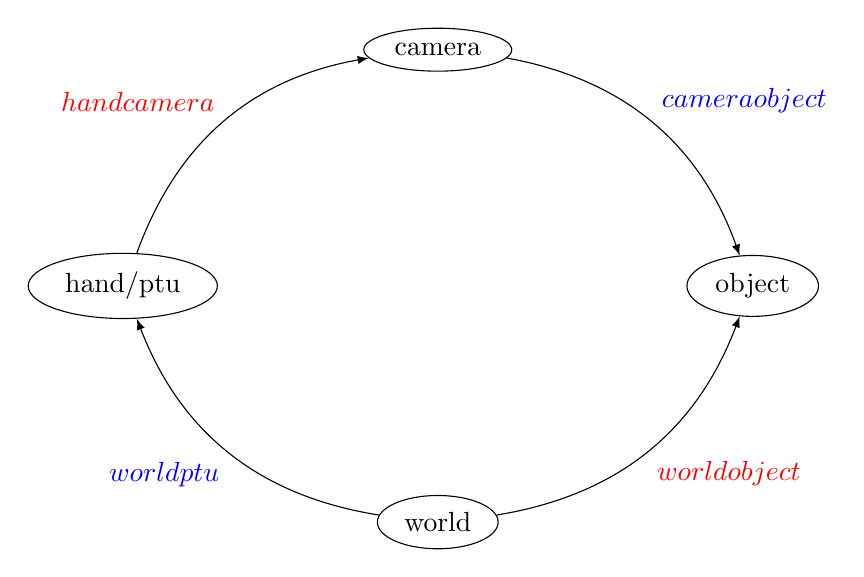
\begin{tikzpicture}
        \node[draw, ellipse] (world) at (0,0) {world};
        \node[draw, ellipse] (hand) at (-4,3) {hand/ptu};
        \node[draw, ellipse] (object) at (4,3) {object};
        \node[draw, ellipse] (camera) at (0, 6) {camera};
        
        \path[-latex]
            (world) edge[bend right] node[midway, below right, red] {$\TF{world}{object}$} (object)
            (world) edge[bend left] node[midway, below left, blue] {$\TF{world}{ptu}$} (hand)
            (hand) edge[bend left] node[midway, above left, red] {$\TF{hand}{camera}$} (camera)
            (camera) edge[bend left] node[midway, above right, blue] {$\TF{camera}{object}$} (object);
    \end{tikzpicture}

    \caption{Hand-in-eye transformation graph}
    \label{fig:hand-in-eye-tf-graph}

\end{figure}

The inspection of the transformation graph determines an equality, because there are two possible ways to transverse the graph from one node to another, which yields the \cref{eqn:hand-in-eye-equality}. This equality is the base of this optimization: $\TF{ptu}{camera}$ can be obtained from multiple pairs of synchronized $\TF{world}{object}$ and $\TF{camera}{object}$ transformations.

\begin{equation}
    \label{eqn:hand-in-eye-equality}
    \TF{world}{object} = \TF{world}{ptu} \cdot \TF{ptu}{camera} \cdot \TF{camera}{object}
\end{equation}

In this work, the object used for detection was an ArUco marker, which is comprised of a pattern which can be detected and also allows for precise pose estimation. One of the biggest advantages over other markers is that the implementation for detection and pose estimation is already implemented in the ROS package \emph{aruco\_detect}. The calibration is also implemented in the ROS package \emph{visp\_hand2eye\_calibration}, as a node that receives multiple transformations in the topics \emph{/world\_effector} and \emph{/camera\_object}, which correspond respectively to the $\TF{world}{ptu}$ and $\TF{camera}{object}$ transformations. To publish the transformations on this topics, a node was developed, the \emph{hand2eye\_simple\_client}, which publishes both the transformations synchronously at the keypress of the user. The control of the PTU was also manual.    

% \input{80-results}
% \input{90-conclusions}

\printbibliography

\end{document}